\documentclass[journal]{IEEEtran}

\usepackage{adjustbox}
\usepackage{algorithm}
\usepackage{algpseudocode}
\usepackage{amsfonts}
\usepackage{amsmath}
\usepackage{amssymb}
\usepackage{amsthm}
\usepackage{array}
% \usepackage{caption}
\usepackage{cite}
\usepackage{colortbl}
\usepackage{environ}
\usepackage{grffile}
\usepackage{hyperref}
\usepackage{import}
\usepackage{mathtools}
\usepackage{microtype}
\usepackage{pgfplots}
\usepackage{siunitx}
\usepackage{stfloats}
\usepackage{tikz}
\usepackage{url}
\usepackage{xcolor}
\usepackage[RPvoltages]{circuitikz}
\usepackage[T1]{fontenc}
\usepackage[caption=false,font=footnotesize]{subfig}
% \usepackage[cmintegrals]{newtxmath}
\usepackage[short]{optidef}


\interdisplaylinepenalty=2500
\pgfplotsset{compat=newest}
\usetikzlibrary{plotmarks}
\usetikzlibrary{arrows.meta}
\usepgfplotslibrary{patchplots}
\newtheorem{proposition}{Proposition}
\newtheorem{remark}{Remark}
\DeclareSIUnit{\belm}{Bm}
\DeclareSIUnit{\dBm}{\deci\belm}
\DeclareSIUnit{\beli}{Bi}
\DeclareSIUnit{\dBi}{\deci\beli}
\usetikzlibrary{arrows,matrix,positioning}


\algrenewcommand{\algorithmicwhile}{\textbf{While}}
\algrenewcommand{\algorithmicif}{\textbf{If}}
\algrenewcommand{\algorithmicthen}{\textbf{Then}}
\algrenewcommand{\algorithmicelse}{\textbf{Else}}
\algrenewcommand{\algorithmicend}{\textbf{End}}
\algrenewcommand{\algorithmicrepeat}{\textbf{Repeat}}
\algrenewcommand{\algorithmicuntil}{\textbf{Until}}


\begin{document}
	\title{Intelligent Reflecting Surface-Aided SWIPT: Joint Waveform, Active and Passive Beamforming Design}
	\author{
		\IEEEauthorblockN{
			Yang~Zhao,~\IEEEmembership{Member,~IEEE,}
			~Bruno~Clerckx,~\IEEEmembership{Senior~Member,~IEEE,}
			and~Zhenyuan~Feng,~\IEEEmembership{Member,~IEEE}
		}
		\thanks{
			The authors are with the Department of Electrical and Electronic Engineering, Imperial College London, London SW7 2AZ, U.K. (e-mail: \{yang.zhao18, b.clerckx, zhenyuan.feng19\}@imperial.ac.uk).

			This paper has been submitted for publication.
		}
	}
	\maketitle


	\begin{abstract}
		The performance of Simultaneous Wireless Information and Power Transfer (SWIPT) is severely restricted by the strength of the received Radio-Frequency (RF) signal. To tackle this problem, we introduce a low-power Intelligent Reflecting Surface (IRS) that compensates the propagation loss and boosts the transmission efficiency by a passive beamforming gain. This paper investigates an efficient IRS-aided SWIPT architecture where a multi-carrier multi-antenna Access Point (AP) transmits information and power simultaneously to a single-antenna User Equipment (UE) under the assist of an IRS. Considering energy harvester nonlinearity, we aim to maximize the Rate-Energy (R-E) tradeoff through a joint optimization of the transmit waveform and active beamforming at the AP, the reflection coefficients at the IRS, and the power splitting ratio at the UE. Stationary solutions are achieved by the Alternating Optimization (AO) technique, where the optimal active beamforming is obtained in closed form, the passive beamforming is optimized by the Successive Convex Approximation (SCA) technique, and the waveform and splitting ratio are optimized by the Geometric Programming (GP) technique. Although practical IRS is limited to Frequency-Flat (FF) reflection, results demonstrate significant benefits of the proposed architecture based on a joint waveform and beamforming design to enlarge the R-E region of IRS-aided SWIPT.
	\end{abstract}


	\begin{IEEEkeywords}
		Simultaneous wireless information and power transfer, intelligent reflecting surface, waveform design, active and passive beamforming.
	\end{IEEEkeywords}


	\begin{section}{Introduction}
		\begin{subsection}{Simultaneous Wireless Information and Power Transfer}
			\IEEEPARstart{W}{ith} the great advance in communication performance, a bottleneck of wireless networks has come to energy supply. Most existing mobile devices are powered by batteries that require frequent charging or replacement, which brings high maintenance cost and restricts the scale of networks. Although solar energy and inductive coupling have become popular alternatives, the former depends on the environment while the latter has a very short operation range. Simultaneous Wireless Information and Power Transfer (SWIPT) is a promising solution to connect and power mobile devices via electromagnetic (EM) waves in the Radio-Frequency (RF) band. It provides low power at \si{\uW} level but broad coverage up to hundreds of meters in a sustainable and controllable manner, bringing more opportunities to the Internet of Things (IoT) and Machine to Machine (M2M) networks. The upsurge in the number of connected devices, together with the decreasing trend in the power consumption of electronics, calls for a re-thinking of future wireless networks based on Wireless Power Transfer (WPT) and SWIPT \cite{Clerckx2019}.

			The concept of SWIPT was first cast in \cite{Varshney2008}, where the authors investigated the Rate-Energy (R-E) tradeoff for a flat Gaussian channel and typical discrete channels. Two co-localized information and power receivers were then proposed in \cite{Zhou2013}, namely Time Switching (TS) that switches between Energy Harvesting (EH) and Information Decoding (ID) modes, and Power Splitting (PS) that splits the received signal into individual components. Dedicated information and energy beamforming were then investigated in \cite{Zhang2013,Park2013} to characterize the R-E region for multi-antenna broadcast and interference channels. On the other hand, \cite{Trotter2009} pointed out that the RF-to-Direct Current (DC) conversion efficiency depends on the input rectifier power and waveform shape. It implies that the modeling of the energy harvester, in particular its nonlinearity, has a crucial and significant impact on the waveform preference, resource allocation and system design of any wireless-powered systems \cite{Trotter2009,Clerckx2018,Clerckx2019}. Motivated by this, \cite{Clerckx2016a} derived a tractable nonlinear harvester model based on the Taylor expansion of diode I-V characteristics, then performed joint waveform and beamforming design for WPT. Simulation and experiments demonstrated that ignoring the energy harvester nonlinearity is inaccurate and emphasized the benefit of modeling such nonlinearity in real system design \cite{Kim2019,Kim2020a}. Importantly, the joint waveform and beamforming strategy for WPT was also shown experimentally in \cite{Kim2020} to be a key technique to expand the operation range. Beyond WPT, the work in \cite{Clerckx2016a} was extended to SWIPT in \cite{Clerckx2018b}, which uniquely showed that the rectifier nonlinearity leads to radical changes to SWIPT design, namely 1) modulated and unmodulated waveforms are not equally suitable for wireless power delivery, 2) a multi-carrier unmodulated waveform superposed to a multi-carrier modulated waveform can enlarge the R-E region of SWIPT, 3) a combination of PS and TS is generally the best strategy, 4) the optimal input distribution is not the conventional Circularly Symmetric Complex Gaussian (CSCG), 5) the rectifier nonlinearity is beneficial to system performance and is essential to efficient SWIPT design. Those observations, validated experimentally in \cite{Kim2019}, led to the question: \textit{What is the optimal input distribution for SWIPT under nonlinearity?} This question was answered in \cite{Varasteh2020} for single-carrier SWIPT, and some attempts were further made in \cite{Varasteh2019d} for multi-carrier SWIPT. The answer sheds new light to fundamental limits of SWIPT and practical signaling (e.g. modulation and waveform) strategies. It is now well understood from \cite{Clerckx2018b,Varasteh2020,Varasteh2019d} that, due to the nonlinearity, a combination of CSCG and on-off keying in single-carrier setting and non-zero mean asymmetric inputs in multi-carrier setting lead to significantly larger R-E region compared to conventional CSCG. Recently, \cite{Varasteh2020a} used machine learning techniques to design SWIPT signaling under nonlinearity to complement the information-theoretic results of \cite{Varasteh2020} and new modulation schemes were subsequently designed.
		\end{subsection}


		\begin{subsection}{Intelligent Reflecting Surface}
			Intelligent Reflecting Surface (IRS) has recently emerged as a promising technique that adapts the wireless channel to increase the spectrum and energy efficiency. In practice, an IRS consists of multiple individual reflecting elements that adjust the amplitude and phase of the incident signal through passive beamforming. Different from relay and backscatter, IRS assists the primary transmission using fully passive components, thus consumes less power with no additional thermal noise but is limited to Frequency-Flat (FF) reflection. Although Frequency-Selective Surface (FSS) has received much attention for wideband communications, it is different from IRS because active FSS requires RF-chains \cite{Kim2006} while passive FSS has fixed physical characteristics and is non-adaptive \cite{Anwar2018}.

			Inspired by the development of real-time reconfigurable metamaterials \cite{Cui2014}, the authors of \cite{Liaskos2018} introduced a programmable metasurface that steers or polarizes the EM wave at a specific frequency to mitigate signal attenuation. Motivated by this, \cite{Wu2018} proposed an IRS-assisted Multiple-Input Single-Output (MISO) system and jointly optimized the precoder at the Access Point (AP) and the phase shifts at the IRS to minimize the transmit power. The active and passive beamforming problem was extended to the discrete phase shift case \cite{Wu2019a} and the multi-user case \cite{Wu2019}. Moreover, \cite{Abeywickrama2019} investigated the coupling effect between reflection amplitude and phase shift based on the impedance equation, and \cite{Nadeem2019} proposed a sequential cascaded channel estimation for Time-Division Duplex (TDD) systems.	A novel dynamic passive beamforming for Orthogonal Frequency-Division Multiplexing (OFDM) systems was proposed in \cite{Yang2020}, which varies the reflection coefficients over consequent slots to enable flexible resource allocation over time-frequency Resource Blocks (RBs). In \cite{Dai2020}, a prototype IRS with \num{256} \num{2}-bit elements based on Positive Intrinsic-Negative (PIN) diodes was developed to support real-time high-definition video transmission at \si{GHz} and mmWave frequency.
		\end{subsection}


		\begin{subsection}{IRS-Aided SWIPT}
			The effective channel enhancement and low power consumption of the IRS are expected to bring more opportunities to SWIPT. For a multi-user IRS-aided SWIPT system, dedicated energy beams are proved unnecessary for the Weighted Sum-Power (WSP) maximization problem \cite{Wu2020b} but essential when considering the fairness issue \cite{Tang2019}. It was also demonstrated in \cite{Wu2020a} that Line-of-Sight (LoS) links can boost the harvested power, where the rank-deficient channels are highly correlated such that a single energy beam can satisfy all energy receivers. However, to the best of our knowledge, all existing IRS-assisted SWIPT papers focus on single-carrier transmission and consider an inaccurate and oversimplified linear energy harvester model. In this paper, we marry the benefits of joint multi-carrier waveform and active beamforming optimization for SWIPT (accounting for nonlinearity) with the passive beamforming capability of the IRS. We ask ourselves the important question: \textit{How to jointly exploit the spatial domain and the frequency domain efficiently through joint waveform and beamforming design to enlarge as much as possible the R-E region of IRS-aided SWIPT?} The contributions of the paper are listed as follows.

			\textit{First}, we introduce a novel IRS-aided SWIPT architecture based on a joint waveform, active and passive beamforming design. This architecture can be seen to IRS-aided SWIPT what \cite{Clerckx2018b} is to SWIPT. Specifically, we consider a IRS-aided multi-carrier downlink MISO SWIPT system where the IRS assists the information and energy transmission of a single user. A multi-carrier unmodulated power waveform (deterministic multisine) is superposed to a multi-carrier modulated information waveform to boost the energy transfer efficiency. The power and information waveforms and the active beamforming at the transmitter, the phase shifts at the IRS, and the splitting ratio at the receiver are jointly optimized to maximize the R-E tradeoff while accounting for the rectenna nonlinearity. This is the first paper to propose such a joint waveform, active and passive beamforming architecture for IRS-aided SWIPT. Note that existing IRS-aided SWIPT papers \cite{Wu2020b,Tang2019,Wu2020a,Pan2020} focus on single-carrier transmissions and ignore the rectenna nonlinearity (and therefore assume the oversimplified and inaccurate linear model \cite{Clerckx2019,Clerckx2016a}), which prevents from exploiting the waveform gain in SWIPT system design. On the contrary, this paper focuses on multi-carrier IRS-SWIPT and investigates the joint design of waveform, active and passive beamforming accounting for rectenna nonlinearity.

			\textit{Second}, we formulate an optimization for this joint waveform, active and passive beamforming design to characterize the R-E region achieved by the proposed architecture. The R-E region characterization problem is transformed into multiple energy maximization problems subject to rate constraints. Each achievable R-E pair is obtained through an Alternating Optimization (AO) algorithm that iteratively updates 1) the phase shift at the IRS, 2) the waveform, active beamforming at the transmitter and the power splitting ratio at the receiver, until convergence. On top of the SWIPT optimization by Geometric Programming (GP) \cite{Clerckx2018b}, our IRS-aided SWIPT optimization employs a low-complexity passive beamforming algorithm based on Successive Convex Approximation (SCA) and Semidefinite Relaxation (SDR), which solves the highly non-convex problem in an efficient and reliable manner. Numerical results demonstrated SDR is tight and the proposed algorithm can always find a stationary point for all tested channel realizations under different configurations.

			\textit{Third}, we conduct numerical evaluations to demonstrate the advantage of the proposed IRS-aided SWIPT architecture. Despite the hardware limitations of the IRS that constraint the reflection elements to be frequency-flat, numerical results show significant R-E benefits of the proposed joint waveform and beamforming design. We confirmed the main observations of SWIPT, namely a dedicated power waveform is beneficial for multi-carrier transmission, and TS/PS are preferred at low/high SNR, carry on to the IRS-aided SWIPT. Moreover, new observations are that 1) the IRS should be placed close to the transmitter or the receiver for optimal performance, 2) the number of transmit antenna and IRS elements have no noticeable impact on the optimal transceiving mode (TS/PS), 3) for active beamforming, increasing the number of transmit antennas brings a linear enhancement to the SNR and a quadratic boost to the harvested DC power, 4) for passive beamforming, increasing the number of reflecting elements provides a quadratic enhancement to the SNR and a quartic boost to the harvested DC power, 5) for narrowband transmission, the optimal active and passive beamforming are fixed for a given channel, and one only need to update the waveform and splitting ratio to draw the whole R-E boundary, 6) for broadband transmission, the frequency diversity enables rate-dependent adaptive passive beamforming to control the subchannel strength distribution and improve the R-E tradeoff.

			\textit{Organization:} The rest of this paper is organized as follows. Section~\ref{se:system_model} introduces the signal, channel, receiver, and R-E tradeoff models of the IRS-aided SWIPT system. Section~\ref{se:problem_formulation} tackles the waveform, active and passive beamforming optimization. Section~\ref{se:performance_evaluation} presents simulation results to evaluate the proposed design. Section~\ref{se:conclusion_and_future_works} concludes the paper.

			\textit{Notations:} Scalars are denoted by italic letters, vectors are denoted by bold lower-case letters, and matrices are denoted by bold upper-case letters. $j$ refers to the imaginary unit. $\mathbb{C}^{x \times y}$ denotes the subspace spanned by complex $x \times y$ matrices. $\Re\{\cdot\}$ and $\Im\{\cdot\}$ stand for the real and imaginary part of a complex number or variable, respectively. $(\cdot)^*$, $(\cdot)^T$ and $(\cdot)^H$ represent the conjugate, transpose, and conjugate transpose operators, respectively. $\mathbb{A}\{\cdot\}$ extracts the DC component of a signal, and $\mathbb{E}_X\{\cdot\}$ takes the expectation over the distribution of the random variable $X$ ($X$ may be omitted for simplicity). For a scalar $x$, $\lvert{x}\rvert$ denotes its absolute value. For a vector $\boldsymbol{x}$, $\lVert{\boldsymbol{x}}\rVert$ refers to its Euclidean norm, $\arg(\boldsymbol{x})$ refers to its argument vector, and $\mathrm{diag}(\boldsymbol{x})$ refers to a square diagonal matrix with the elements of $\boldsymbol{x}$ on the main diagonal. For a general matrix $\boldsymbol{M}$, $\mathrm{rank}(\boldsymbol{M})$ denotes it rank. For a square matrix $\boldsymbol{S}$, $\mathrm{Tr}(\boldsymbol{S})$ denotes its trace, and $\boldsymbol{S} \succeq 0$ means that $\boldsymbol{S}$ is positive semi-definite. The distribution of a CSCG random vector with mean vector $\boldsymbol{0}$ and covariance matrix $\boldsymbol{\Sigma}$ is denoted by $\mathcal{CN}(\boldsymbol{0},\boldsymbol{\Sigma})$, and $\sim$ stands for "distributed as". We also denote $(\cdot)^{\star}$ and $(\cdot)^{(i)}$ as the stationary solution and the solution at iteration $i$, respectively.
		\end{subsection}
	\end{section}


	\begin{section}{System Model}\label{se:system_model}
		\begin{figure}[!t]
			\centering
			\def\svgwidth{0.9\columnwidth}
			\import{assets/}{system.pdf_tex}
			\caption{An IRS-aided multi-carrier SWIPT system.}
			\label{fi:system}
		\end{figure}

		As shown in Fig.~\ref{fi:system}, we propose an IRS-aided SWIPT system where a $M$-antenna AP delivers information and power simultaneously, through a $L$-element IRS, to a single-antenna User Equipment (UE) over $N$ orthogonal evenly-spaced subbands. We consider a quasi-static block fading model and focus on an instance where all channels are constant. The AP is assumed to have partial or perfect Channel State Information (CSI) of the AP-UE channel and the cascaded AP-IRS-UE channel. We also omit the signals reflected two and more times and assume the noise power is too small to be harvested.


		\begin{subsection}{Transmitted Signal}
			Denote $\tilde{x}_{\mathrm{I},n}\sim\mathcal{CN}(0,1)$ as the information symbol transmitted over subband $n \in \{1, \dots, N\}$. The superposed signal transmitted on antenna $m \in \{1, \dots, M\}$ at time $t$ is
			\begin{equation}\label{eq:x_m}
				x_m(t)=\Re\left\{\sum_{n=1}^N\left({w_{\mathrm{I},n,m}\tilde{x}_{\mathrm{I},n}(t)}+w_{\mathrm{P},n,m}\right){e^{j2{\pi}{f_n}{t}}}\right\}
			\end{equation}
			where $w_{\mathrm{I/P},n,m}$ denotes the complex weight of the modulated/multisine waveform transmitted at subband $n$ on antenna $m$, and $f_n$ is the frequency of subband $n$. On top of this, we stack up $\boldsymbol{w}_{\mathrm{I/P},n} \triangleq [w_{\mathrm{I/P},n,1},\dots,w_{\mathrm{I/P},n,M}]^T \in \mathbb{C}^{M \times 1}$ and $\boldsymbol{x}(t) \triangleq [x_1(t),\dots,x_M(t)]^T \triangleq \boldsymbol{x}_{\mathrm{I}}(t)+\boldsymbol{x}_{\mathrm{P}}(t) \in \mathbb{C}^{M \times 1}$, where
			\begin{align}
				\boldsymbol{x}_{\mathrm{I}}(t) &= \Re{\left\{\sum_{n=1}^N\boldsymbol{w}_{\mathrm{I},n}\tilde{x}_{\mathrm{I},n}(t){e^{j2{\pi}{f_n}{t}}}\right\}},\label{eq:x_I}\\
				\boldsymbol{x}_{\mathrm{P}}(t) &= \Re{\left\{\sum_{n=1}^N\boldsymbol{w}_{\mathrm{P},n}{e^{j2{\pi}{f_n}{t}}}\right\}}\label{eq:x_P}
			\end{align}
			are the modulated and multisine components, respectively.
		\end{subsection}


		\begin{subsection}{Reflection Pattern and Composite Channel}
			Green's decomposition \cite{Hansen1989} suggests that the backscattered signal of an antenna can be decomposed into the \emph{structural mode} component and the \emph{antenna mode} component. The former is fixed for a given antenna and can be regarded as part of the environment multipath, while the latter is adjustable and depends on the mismatch of the antenna and load impedances. IRS element $l \in \{1, \dots, L\}$ varies its impedance $Z_l = R_l + j X_l$ in a fully passive manner to reflect the incoming signal, and the reflection coefficient is defined as
			\begin{equation}
				\phi_l = \frac{Z_l - Z_0}{Z_l + Z_0} \triangleq \eta_l e^{j\theta_l}
			\end{equation}
			where $Z_0$ is the characteristic impedance, $\eta_l \in [0, 1]$ is the reflection amplitude, and $\theta_l \in [0,2\pi)$ is the phase shift~\footnote{Due to the non-zero power consumption at the IRS, practically $R_l > 0$ such that $\eta_l < 1$ and depends on $\theta_l$. This paper sticks to the commonest and simplest IRS model where the reflection coefficient is assumed unit.}. We also denote $\boldsymbol{\Theta} \triangleq \mathrm{diag}(\phi_1, \dots, \phi_L) \in \mathbb{C}^{L \times L}$ as the IRS matrix and define $\boldsymbol{\phi} \triangleq [\phi_1, \dots, \phi_L]^H \in \mathbb{C}^{L \times 1}$ as the IRS vector~\footnote{Note the conjugate transpose in the notation of $\boldsymbol{\phi}$ makes its entries the complex conjugate of the diagonal entries of $\boldsymbol{\Theta}$.}.

			\begin{remark}\label{re:reflection_coefficient}
				The element impedance $Z_l$ maps to the reflection coefficient $\phi_l$ uniquely. Since the reactance $X_l$ depends on frequency, the reflection coefficient $\phi_l$ is also a function of frequency and cannot be designed independently at different subbands. In this paper, we assume the bandwidth is incomparable to the operating frequency such that the reflection coefficients of each IRS element are the same at all subbands. That is to say, $\phi_l$ is shared by $M$ AP-IRS-UE channels over $N$ subbands.
			\end{remark}

			At subband $n$, we denote the AP-UE direct channel as $\boldsymbol{h}_{\mathrm{D},n}^H \in \mathbb{C}^{1 \times M}$, AP-IRS incident channel as $\boldsymbol{H}_{\mathrm{I},n} \in \mathbb{C}^{L \times M}$, and IRS-UE reflective channel as $\boldsymbol{h}_{\mathrm{R},n}^H \in \mathbb{C}^{1 \times L}$. The auxiliary link provided by the IRS can be modeled as a concatenation of the incident channel, the IRS reflection, and the reflective channel. Therefore, the composite equivalent channel reduces to
			\begin{equation}\label{eq:h_n}
				\boldsymbol{h}_{n}^H = \boldsymbol{h}_{\mathrm{D},n}^H + \boldsymbol{h}_{\mathrm{R},n}^H \boldsymbol{\Theta} \boldsymbol{H}_{\mathrm{I},n} = \boldsymbol{h}_{\mathrm{D},n}^H + \boldsymbol{\phi}^H \boldsymbol{V}_{n}
			\end{equation}
			where we define $\boldsymbol{V}_{n} \triangleq \mathrm{diag}(\boldsymbol{h}_{\mathrm{R},n}^H)\boldsymbol{H}_{\mathrm{I},n} \in \mathbb{C}^{L \times M}$.
		\end{subsection}


		\begin{subsection}{Received Signal}
			The total received signal at the single-antenna UE can be decomposed as $y(t) \triangleq y_{\mathrm{I}}(t)+y_\mathrm{P}(t)$, where
			\begin{align}
				y_{\mathrm{I}}(t) & = \Re\left\{\sum_{n=1}^N{\boldsymbol{h}_{n}^H}{\boldsymbol{w}_{\mathrm{I},n}\tilde{x}_{\mathrm{I},n}(t)}{e^{j2{\pi}{f_n}{t}}}\right\},\label{eq:y_I}\\
				y_{\mathrm{P}}(t) & = \Re\left\{\sum_{n=1}^N{\boldsymbol{h}_{n}^H}\boldsymbol{w}_{\mathrm{P},n}{e^{j2{\pi}{f_n}{t}}}\right\}\label{eq:y_P}
			\end{align}
			capture the contribution of modulated and multisine waveforms over all subbands. Note that $y_{\mathrm{I}}(t)$ can also be used for energy harvesting if necessary, but $y_{\mathrm{P}}(t)$ is unmodulated and cannot be used for information purpose.
		\end{subsection}


		\begin{subsection}{Transceiving Modes}
			Consider TS and PS as two practical transceiving modes in the SWIPT system design. TS relies on perfect clock synchronization, where the transmitter divides each slot into dedicated data session with length $1 - \eta$ and energy session with length $\eta$, then designs the waveform for WIT and WPT independently. At the receiver end, only information decoder or energy harvester would be activated in the corresponding session. Varying $\eta$ from \num{0} to \num{1} corresponds to a R-E segment from WIT point to WPT point.

			On the other hand, the PS transmitter optimizes the superposed waveform that remains unchanged in the entire slot, and the receiver splits the incoming signal into individual data stream with power proportion $1 - \rho$ and energy stream with power proportion $\rho$. Note that in PS the splitting ratio $\rho$ and the superposed waveform are coupled thus require a joint design, but in TS the duration ratio $\eta$ is irrelevant to the waveform design in both sessions. Therefore, we focus on PS in the following context since TS can be obtained by a direct time sharing between WIT and WPT.
		\end{subsection}


		\begin{subsection}{Information Decoder}
			A major benefit of the superposed waveform is that the multisine is deterministic and creates no interference to the modulated waveform. Therefore, the achievable rate writes as
			\begin{equation}\label{eq:R}
				R(\boldsymbol{\phi},\boldsymbol{w}_{\mathrm{I}},\rho) = \sum_{n=1}^N{\log_2\left(1+\frac{(1-\rho)\lvert \boldsymbol{h}_{n}^H\boldsymbol{w}_{\mathrm{I},n} \rvert^2}{\sigma_n^2}\right)}
			\end{equation}
			where $\rho$ is the power splitting ratio for the energy harvester, $\sigma_n^2$ is the variance of the total noise (at RF-band and during RF-to-baseband conversion) on tone $n$. Rate \eqref{eq:R} is achievable with either waveform cancellation or translated demodulation \cite{Clerckx2018b}.
		\end{subsection}


		\begin{subsection}{Energy Harvester}
			\begin{figure}[!t]
				\centering
				\subfloat[Antenna equivalent circuit\label{ci:antenna_equivalent_circuit}]{
					\resizebox{0.45\columnwidth}{!}{
						\begin{circuitikz}[transform shape]
							\draw (0,0) to [sV=$v_{\mathrm{S}}$] (0,2);
							\draw (0,2) to [short] (1,2);
							\draw (1,2) to [R=$R_{\mathrm{A}}$] (3,2);
							\draw (3,2) to [short] (4,2);
							\draw (4,2) to [R=$R_{\mathrm{in}}$, v<=$v_{\mathrm{in}}$] (4,0);
							\draw (4,0) to [short] (2,0) node[ground](GND){};
							\draw (2,0) to [short] (0,0);
						\end{circuitikz}
					}
				}
				\subfloat[A single diode rectifier\label{ci:single_diode_rectifier}]{
					\resizebox{0.45\columnwidth}{!}{
						\begin{circuitikz}[transform shape]
							\draw (0,0) to [sV=$v_{\mathrm{in}}$] (0,2);
							\draw (0,2) to [short] (0.25,2);
							\draw (0.25,2) to [D, v<=$v_{\mathrm{D}}$, i=$i_{\mathrm{D}}$] (2.25,2);
							\draw (2.25,2) to [short, -*] (2.5,2);
							\draw (2.5,2) to [C, l_=$C$, -*] (2.5,0);
							\draw (2.5,2) to [short] (4,2);
							\draw (4,2) to [R=$R_{\mathrm{L}}$, v<=$v_{\mathrm{out}}$, i=$i_{\mathrm{out}}$] (4,0);
							\draw (4,0) to [short] (2,0) node[ground](GND){};
							\draw (2,0) to [short] (0,0);
						\end{circuitikz}
					}
				}
				\caption{Receive antenna and energy harvester circuits.}
			\end{figure}

			In this section, we briefly revisit a tractable nonlinear rectenna model that relates the harvester output DC current to the received signal. Fig.~\ref{ci:antenna_equivalent_circuit} illustrates the equivalent circuit of an ideal antenna, where the antenna has an impedance $R_{\mathrm{A}}$ and the incoming signal creates an voltage source $v_{\mathrm{S}}(t)$. Let $R_{\mathrm{in}}$ be the total input impedance of the rectifier and matching network, and we assume the voltage across the matching network is negligible. When perfectly matched ($R_{\mathrm{in}}=R_{\mathrm{A}}$), the rectifier input voltage is $v_{\mathrm{in}}(t)=y(t)\sqrt{\rho R_{\mathrm{A}}}$.

			Rectifiers consist of nonlinear components as diode and capacitor to produce DC output and store energy \cite{Pinuela2013}. Consider a simplified rectifier model in Fig.~\ref{ci:single_diode_rectifier} where a single series diode is followed by a low-pass filter with a parallel load. As detailed in \cite{Clerckx2016a,Clerckx2018b}, a truncated Taylor expansion of the diode I-V characteristic equation suggests that, when the subband frequencies are evenly-spaced, maximizing the average output DC current is equivalent to maximizing a monotonic function \footnote{Note that this small-signal expansion model is only valid for the non-linear operation region of the diode, and the I-V relationship would be linear if the diode behavior is dominated by the load \cite{Clerckx2016a}.}
			\begin{equation}\label{eq:z}
				z(\boldsymbol{\phi},\boldsymbol{w}_{\mathrm{I}},\boldsymbol{w}_{\mathrm{P}},\rho)=\sum_{i\,\mathrm{even},i\ge2}^{n_0}{k_i}{\rho^{i/2}}{R_{\mathrm{A}}^{i/2}}{\mathbb{E}\left\{\mathbb{A}\left\{y(t)^i\right\}\right\}}
			\end{equation}
			where $n_0$ is the truncation order and $k_i \triangleq i_{\mathrm{S}}/i!(n'v_{\mathrm{T}})^i$ is the diode coefficient ($i_{\mathrm{S}}$ is the reverse bias saturation current, $n'$ is the diode ideality factor, $v_{\mathrm{T}}$ is the thermal voltage). With a slight abuse of notation, we refer to $z$ as the average output DC current in the following context. It can be observed that the traditional linear harvester model, where the output DC power equals the sum of the power harvested on each frequency, is a special case of \eqref{eq:z} with $n_0=2$. However, due to the coupling effect among different frequencies, some high-order AC components compensate each other and further contribute to the output DC power. In other words, even-order terms with $i \ge 4$ account for the diode nonlinear behavior. For simplicity, we choose $n_0=4$ to investigate the fundamental rectifier nonlinearity, and define $\beta_2 \triangleq {k_2}{R_{\mathrm{A}}}$, $\beta_4 \triangleq {k_4}{R_{\mathrm{A}}^2}$ to rewrite $z$ by \eqref{eq:z_expand}. Note that $\mathbb{E}\left\{\lvert\tilde{x}_{\mathrm{I},n}\rvert^2\right\}=1$ but $\mathbb{E}\left\{\lvert\tilde{x}_{\mathrm{I},n}\rvert^4\right\}=2$, which can be interpreted as a modulation gain on the nonlinear terms of the output DC current. Inspired by \cite{Huang2017}, we further stack $\boldsymbol{h} \triangleq [\boldsymbol{h}_1^T,\dots,\boldsymbol{h}_N^T]^T \in \mathbb{C}^{MN \times 1}$, $\boldsymbol{w}_{\mathrm{I/P}} \triangleq [\boldsymbol{w}_{\mathrm{I/P},1}^T,\dots,\boldsymbol{w}_{\mathrm{I/P},N}^T]^T \in \mathbb{C}^{MN \times 1}$, and define $\boldsymbol{W}_{\mathrm{I/P}} \triangleq \boldsymbol{w}_{\mathrm{I/P}}\boldsymbol{w}_{\mathrm{I/P}}^H \in \mathbb{C}^{MN \times MN}$. As illustrated by Fig.~\ref{fi:block_diagonal}, $\boldsymbol{W}_{\mathrm{I/P}}$ can be divided into $N \times N$ blocks of size $M \times M$, and we let $\boldsymbol{W}_{\mathrm{I/P},k}$ keep its $k$-th ($k=-N+1,\dots,N-1$) block diagonal and set all other blocks to $\boldsymbol{0}^{M \times M}$. Hence, the components of the average output DC current $z$ can be expressed in \eqref{eq:y_I2} -- \eqref{eq:y_P4}.

			\begin{figure*}[!t]
				\begin{equation*}
						\boldsymbol{W}_{\mathrm{I/P}}=
						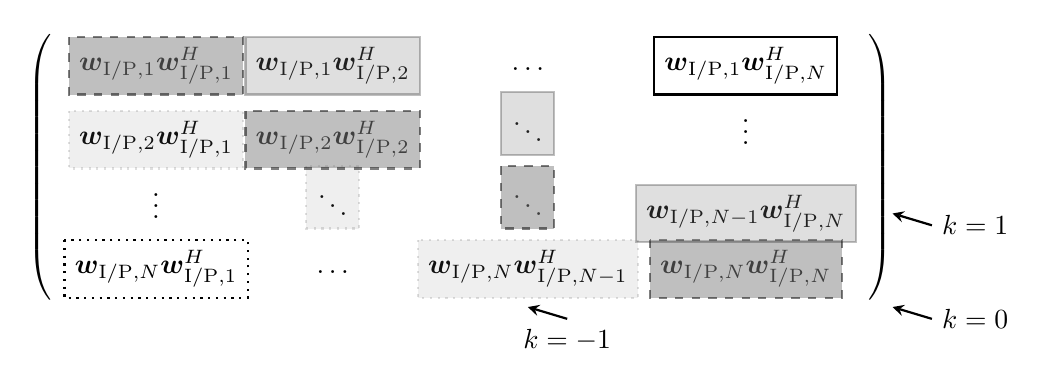
\begin{tikzpicture}[>=stealth,thick,baseline,every right delimiter/.append style={name=rd},]
							\matrix [matrix of math nodes,left delimiter=(,right delimiter=)] (m)
							{
								\boldsymbol{w}_{\mathrm{I/P},1}\boldsymbol{w}_{\mathrm{I/P},1}^H & \boldsymbol{w}_{\mathrm{I/P},1}\boldsymbol{w}_{\mathrm{I/P},2}^H & \dots & \boldsymbol{w}_{\mathrm{I/P},1}\boldsymbol{w}_{\mathrm{I/P},N}^H \\
								\boldsymbol{w}_{\mathrm{I/P},2}\boldsymbol{w}_{\mathrm{I/P},1}^H & \boldsymbol{w}_{\mathrm{I/P},2}\boldsymbol{w}_{\mathrm{I/P},2}^H & \ddots & \vdots \\
								\vdots & \ddots & \ddots & \boldsymbol{w}_{\mathrm{I/P},N-1}\boldsymbol{w}_{\mathrm{I/P},N}^H \\
								\boldsymbol{w}_{\mathrm{I/P},N}\boldsymbol{w}_{\mathrm{I/P},1}^H & \dots & \boldsymbol{w}_{\mathrm{I/P},N}\boldsymbol{w}_{\mathrm{I/P},N-1}^H & \boldsymbol{w}_{\mathrm{I/P},N}\boldsymbol{w}_{\mathrm{I/P},N}^H \\
							};
							\draw[dotted,thick] (m-4-1.north west) rectangle (m-4-1.south east);
							\draw[dotted,thick,fill=gray,opacity=0.125] (m-2-1.north west) rectangle (m-2-1.south east); \draw[dotted,thick,fill=gray,opacity=0.125] (m-3-2.north west) rectangle (m-3-2.south east); \draw[dotted,thick,fill=gray,opacity=0.125] (m-4-3.north west) rectangle (m-4-3.south east);
							\draw[dashed,thick,fill=gray,opacity=0.5] (m-1-1.north west) rectangle (m-1-1.south east); \draw[dashed,thick,fill=gray,opacity=0.5] (m-2-2.north west) rectangle (m-2-2.south east); \draw[dashed,thick,fill=gray,opacity=0.5] (m-3-3.north west) rectangle (m-3-3.south east); \draw[dashed,thick,fill=gray,opacity=0.5] (m-4-4.north west) rectangle (m-4-4.south east);
							\draw[solid,thick,fill=gray,opacity=0.25] (m-1-2.north west) rectangle (m-1-2.south east); \draw[solid,thick,fill=gray,opacity=0.25] (m-2-3.north west) rectangle (m-2-3.south east); \draw[solid,thick,fill=gray,opacity=0.25] (m-3-4.north west) rectangle (m-3-4.south east);
							\draw[solid,thick] (m-1-4.north west) rectangle (m-1-4.south east);
							\draw[<-] (m-4-3.south|-m.south) -- ++(0.5,-0.15) node[below]{$k=-1$};
							\draw[<-] (rd.east|-m.south) -- ++(0.5,-0.15) node[right]{$k=0$};
							\draw[<-] (rd.east|-m-3-4.east) -- ++(0.5,-0.15) node[right]{$k=1$};
						\end{tikzpicture}
				\end{equation*}
				\caption{$\boldsymbol{W}_{\mathrm{I/P}}$ consists of $N \times N$ blocks of size $M \times M$. $\boldsymbol{W}_{\mathrm{I/P},k}$ keeps the $k$-th block diagonal of $\boldsymbol{W}_{\mathrm{I/P}}$ and nulls all remaining blocks. Solid, dashed and dotted blocks correspond to $k>0$, $k=0$ and $k<0$, respectively. For $\boldsymbol{w}_{\mathrm{I/P},n_1}\boldsymbol{w}_{\mathrm{I/P},n_2}^H$, the $k$-th block diagonal satisfies $k=n_2-n_1$.}
				\label{fi:block_diagonal}
			\end{figure*}

			\begin{figure*}[!b]
				\hrule
				\begin{equation}
					z(\boldsymbol{\phi},\boldsymbol{w}_{\mathrm{I}},\boldsymbol{w}_{\mathrm{P}},\rho) = \beta_2\rho\Bigl(\mathbb{E}\left\{\mathbb{A}\left\{y_{\mathrm{I}}^2(t)\right\}\right\}+\mathbb{A}\left\{y_{\mathrm{P}}^2(t)\right\}\Bigr)+\beta_4\rho^2\Bigl(\mathbb{E}\left\{\mathbb{A}\left\{y_{\mathrm{I}}^4(t)\right\}\right\}+\mathbb{A}\left\{y_{\mathrm{P}}^4(t)\right\}+6\mathbb{E}\left\{\mathbb{A}\left\{y_{\mathrm{I}}^2(t)\right\}\right\}\mathbb{A}\left\{y_{\mathrm{P}}^2(t)\right\}\Bigr).\label{eq:z_expand}
				\end{equation}
				\hrule
				\begin{flalign}
					\mathbb{E}\left\{\mathbb{A}\left\{y_{\mathrm{I}}^2(t)\right\}\right\}
					& = \frac{1}{2}\sum_{n=1}^N{(\boldsymbol{h}_{n}^H\boldsymbol{w}_{\mathrm{I},n})(\boldsymbol{h}_{n}^H\boldsymbol{w}_{\mathrm{I},n})^*} = \frac{1}{2}\boldsymbol{h}^H\boldsymbol{W}_{\mathrm{I},0}\boldsymbol{h},&&\label{eq:y_I2}\\
					\mathbb{E}\left\{\mathbb{A}\left\{y_{\mathrm{I}}^4(t)\right\}\right\}
					& = \frac{3}{4}\left(\sum_{n=1}^N{(\boldsymbol{h}_{n}^H\boldsymbol{w}_{\mathrm{I},n})(\boldsymbol{h}_{n}^H\boldsymbol{w}_{\mathrm{I},n})^*}\right)^2 = \frac{3}{4}(\boldsymbol{h}^H\boldsymbol{W}_{\mathrm{I},0}\boldsymbol{h})^2,&&\label{eq:y_I4}
				\end{flalign}
				\begin{flalign}
					\mathbb{A}\left\{y_{\mathrm{P}}^2(t)\right\}
					& = \frac{1}{2}\sum_{n=1}^N{(\boldsymbol{h}_{n}^H\boldsymbol{w}_{\mathrm{P},n})(\boldsymbol{h}_{n}^H\boldsymbol{w}_{\mathrm{P},n})^*} = \frac{1}{2}\boldsymbol{h}^H\boldsymbol{W}_{\mathrm{P},0}\boldsymbol{h},&&\label{eq:y_P2}\\
					\mathbb{A}\left\{y_{\mathrm{P}}^4(t)\right\}
					& = \frac{3}{8}\sum_{\substack{{n_1},{n_2},{n_3},{n_4}\\{n_1}+{n_2}={n_3}+{n_4}}}{(\boldsymbol{h}_{{n_1}}^H\boldsymbol{w}_{\mathrm{P},{n_1}})(\boldsymbol{h}_{{n_2}}^H\boldsymbol{w}_{\mathrm{P},{n_2}})(\boldsymbol{h}_{{n_3}}^H\boldsymbol{w}_{\mathrm{P},{n_3}})^*(\boldsymbol{h}_{{n_4}}^H\boldsymbol{w}_{\mathrm{P},{n_4}})^*} = \frac{3}{8}\sum_{k=-N+1}^{N-1}(\boldsymbol{h}^H\boldsymbol{W}_{\mathrm{P},k}\boldsymbol{h})(\boldsymbol{h}^H\boldsymbol{W}_{\mathrm{P},k}\boldsymbol{h})^*.&&\label{eq:y_P4}
				\end{flalign}
			\end{figure*}
			% \begin{figure*}[!b]
			% 	\hrule
			% 	\begin{align}
			% 		z(\boldsymbol{\phi},\boldsymbol{w}_{\mathrm{I}},\boldsymbol{w}_{\mathrm{P}},\rho) & = \beta_2\rho\Bigl(\mathbb{E}\left\{\mathbb{A}\left\{y_{\mathrm{I}}^2(t)\right\}\right\}+\mathbb{A}\left\{y_{\mathrm{P}}^2(t)\right\}\Bigr)\nonumber\\
			% 		& \quad + \beta_4\rho^2\Bigl(\mathbb{E}\left\{\mathbb{A}\left\{y_{\mathrm{I}}^4(t)\right\}\right\}+\mathbb{A}\left\{y_{\mathrm{P}}^4(t)\right\}+6\mathbb{E}\left\{\mathbb{A}\left\{y_{\mathrm{I}}^2(t)\right\}\right\}\mathbb{A}\left\{y_{\mathrm{P}}^2(t)\right\}\Bigr).\label{eq:z_expand}
			% 	\end{align}
			% 	\hrule
			% 	\begin{align}
			% 		\mathbb{E}\left\{\mathbb{A}\left\{y_{\mathrm{I}}^2(t)\right\}\right\}
			% 		& = \frac{1}{2}\sum_{n=1}^N{(\boldsymbol{h}_{n}^H\boldsymbol{w}_{\mathrm{I},n})(\boldsymbol{h}_{n}^H\boldsymbol{w}_{\mathrm{I},n})^*} = \frac{1}{2}\boldsymbol{h}^H\boldsymbol{W}_{\mathrm{I},0}\boldsymbol{h},\label{eq:y_I2}\\
			% 		\mathbb{E}\left\{\mathbb{A}\left\{y_{\mathrm{I}}^4(t)\right\}\right\}
			% 		& = \frac{3}{4}\left(\sum_{n=1}^N{(\boldsymbol{h}_{n}^H\boldsymbol{w}_{\mathrm{I},n})(\boldsymbol{h}_{n}^H\boldsymbol{w}_{\mathrm{I},n})^*}\right)^2 = \frac{3}{4}(\boldsymbol{h}^H\boldsymbol{W}_{\mathrm{I},0}\boldsymbol{h})^2,\label{eq:y_I4}\\
			% 		\mathbb{A}\left\{y_{\mathrm{P}}^2(t)\right\}
			% 		& = \frac{1}{2}\sum_{n=1}^N{(\boldsymbol{h}_{n}^H\boldsymbol{w}_{\mathrm{P},n})(\boldsymbol{h}_{n}^H\boldsymbol{w}_{\mathrm{P},n})^*} = \frac{1}{2}\boldsymbol{h}^H\boldsymbol{W}_{\mathrm{P},0}\boldsymbol{h},\label{eq:y_P2}\\
			% 		\mathbb{A}\left\{y_{\mathrm{P}}^4(t)\right\}
			% 		& = \frac{3}{8}\sum_{\substack{{n_1},{n_2},{n_3},{n_4}\\{n_1}+{n_2}={n_3}+{n_4}}}{(\boldsymbol{h}_{{n_1}}^H\boldsymbol{w}_{\mathrm{P},{n_1}})(\boldsymbol{h}_{{n_2}}^H\boldsymbol{w}_{\mathrm{P},{n_2}})(\boldsymbol{h}_{{n_3}}^H\boldsymbol{w}_{\mathrm{P},{n_3}})^*(\boldsymbol{h}_{{n_4}}^H\boldsymbol{w}_{\mathrm{P},{n_4}})^*}\nonumber\\
			% 		& = \frac{3}{8}\sum_{k=-N+1}^{N-1}(\boldsymbol{h}^H\boldsymbol{W}_{\mathrm{P},k}\boldsymbol{h})(\boldsymbol{h}^H\boldsymbol{W}_{\mathrm{P},k}\boldsymbol{h})^*.\label{eq:y_P4}
			% 	\end{align}
			% \end{figure*}
		\end{subsection}


		\begin{subsection}{Rate-Energy Region}
			The achievable R-E region is defined as
			\begin{align}
				C_{R_{\mathrm{ID}}-I_{\mathrm{EH}}}(P)
				&\triangleq \biggl\{(R_{\mathrm{ID}}, I_{\mathrm{EH}}): R_{\mathrm{ID}} \le R, I_{\mathrm{EH}} \le z,\nonumber\\
				&\quad \frac{1}{2}\left(\lVert{\boldsymbol{w}_{\mathrm{I}}}\rVert^2+\lVert{\boldsymbol{w}_{\mathrm{P}}}\rVert^2\right) \le P\biggr\}
			\end{align}
			% \begin{equation}
			% 	C_{R_{\mathrm{ID}}-I_{\mathrm{EH}}}(P) \triangleq \biggl\{(R_{\mathrm{ID}}, I_{\mathrm{EH}}): R_{\mathrm{ID}} \le R, I_{\mathrm{EH}} \le z, \frac{1}{2}\left(\lVert{\boldsymbol{w}_{\mathrm{I}}}\rVert^2+\lVert{\boldsymbol{w}_{\mathrm{P}}}\rVert^2\right) \le P\biggr\}
			% \end{equation}
			where $P$ is the average transmit power budget and the coefficient \num{1/2} converts the peak power of sinewaves to the average power.
		\end{subsection}
	\end{section}


	\begin{section}{Problem Formulation}\label{se:problem_formulation}
		We characterize the R-E region through a current maximization problem subject to transmit power, IRS magnitude, and rate constraints
		\begin{maxi!}
			{\boldsymbol{\phi},\boldsymbol{w}_{\mathrm{I}},\boldsymbol{w}_{\mathrm{P}},\rho}{z(\boldsymbol{\phi},\boldsymbol{w}_{\mathrm{I}},\boldsymbol{w}_{\mathrm{P}},\rho)}{\label{op:original}}{\label{ob:original}}
			\addConstraint{\frac{1}{2}\left(\lVert{\boldsymbol{w}_{\mathrm{I}}}\rVert^2+\lVert{\boldsymbol{w}_{\mathrm{P}}}\rVert^2\right)\le{P}}\label{co:original_power}
			\addConstraint{R(\boldsymbol{\phi},\boldsymbol{w}_{\mathrm{I}},\rho) \ge \bar{R}}\label{co:original_rate}
			\addConstraint{\lvert{\phi_l}\rvert=1, \quad l=1,\dots,L}\label{co:original_modulus}
			\addConstraint{0 \le \rho \le 1.}
		\end{maxi!}
		Problem~\eqref{op:original} is intricate with coupled variables in non-convex expressions \eqref{ob:original}, \eqref{co:original_rate}, \eqref{co:original_modulus}. To obtain a feasible solution, we propose an AO algorithm that iteratively updates 1) the phase shift at the IRS, 2) the waveform, active beamforming at the transmitter and the power splitting ratio at the receiver, until convergence.
		\begin{remark}\label{re:irs_subchannel_alignment}
			As information and power transfer prefer different subchannel strength distribution, the frequency-flat characteristic of the IRS introduces a resource allocation problem. Following Remark~\ref{re:irs_frequency_flat}, if the IRS is frequency-selective and there is only one transmit antenna, then each reflecting element can simultaneously align the corresponding AP-IRS-UE channel with the AP-UE channel at all subbands. In this case, the strengths of all subchannels are maximized so that the joint design would follow straightforwardly from existing SWIPT work \cite{Clerckx2018b}.
		\end{remark}


		\begin{subsection}{Passive Beamforming}
			In this section, we optimize the IRS phase shift $\boldsymbol{\phi}$ for any given waveform $\boldsymbol{w}_{\mathrm{I/P}}$ and splitting ratio $\rho$. Note that
			\begin{align}
				\lvert \boldsymbol{h}_{n}^H\boldsymbol{w}_{\mathrm{I},n} \rvert^2
				& = \boldsymbol{w}_{\mathrm{I},n}^H\boldsymbol{h}_n\boldsymbol{h}_n^H\boldsymbol{w}_{\mathrm{I},n}\nonumber\\
				& = \boldsymbol{w}_{\mathrm{I},n}^H(\boldsymbol{h}_{\mathrm{D},n}+\boldsymbol{V}_n^H\boldsymbol{\phi})(\boldsymbol{h}_{\mathrm{D},n}^H+\boldsymbol{\phi}^H\boldsymbol{V}_n)\boldsymbol{w}_{\mathrm{I},n}\nonumber\\
				& = \boldsymbol{w}_{\mathrm{I},n}^H\boldsymbol{M}_n^H\boldsymbol{\Phi}\boldsymbol{M}_n\boldsymbol{w}_{\mathrm{I},n}\nonumber\\
				& = \mathrm{Tr}(\boldsymbol{M}_n\boldsymbol{w}_{\mathrm{I},n}\boldsymbol{w}_{\mathrm{I},n}^H\boldsymbol{M}_n^H\boldsymbol{\Phi})\nonumber\\
				& = \mathrm{Tr}(\boldsymbol{C}_n\boldsymbol{\Phi})
			\end{align}
			where $\boldsymbol{M}_n \triangleq [\boldsymbol{V}_n^H, \boldsymbol{h}_{\mathrm{D},n}]^H \in \mathbb{C}^{(L+1) \times M}$, $t$ is an auxiliary variable with unit modulus, $\bar{\boldsymbol{\phi}} \triangleq [\boldsymbol{\phi}^H, t]^H \in \mathbb{C}^{(L+1) \times 1}$, $\boldsymbol{\Phi} \triangleq \bar{\boldsymbol{\phi}}\bar{\boldsymbol{\phi}}^H \in \mathbb{C}^{(L+1) \times (L+1)}$, $\boldsymbol{C}_n \triangleq \boldsymbol{M}_n\boldsymbol{w}_{\mathrm{I},n}\boldsymbol{w}_{\mathrm{I},n}^H\boldsymbol{M}_n^H \in \mathbb{C}^{(L+1)\times(L+1)}$. On the other hand, we define $t_{\mathrm{I/P},k}$ as
			\begin{align}
				t_{\mathrm{I/P},k}
				& \triangleq \boldsymbol{h}^H\boldsymbol{W}_{\mathrm{I/P},k}\boldsymbol{h}\nonumber\\
				& = \mathrm{Tr}(\boldsymbol{h}\boldsymbol{h}^H\boldsymbol{W}_{\mathrm{I/P},k})\nonumber\\
				& = \mathrm{Tr}\left((\boldsymbol{h}_{D}+\boldsymbol{V}^H\boldsymbol{\phi})(\boldsymbol{h}_{D}^H+\boldsymbol{\phi}^H\boldsymbol{V})\boldsymbol{W}_{\mathrm{I/P},k}\right)\nonumber\\
				& = \mathrm{Tr}(\boldsymbol{M}^H\boldsymbol{\Phi}\boldsymbol{M}\boldsymbol{W}_{\mathrm{I/P},k})\nonumber\\
				& = \mathrm{Tr}(\boldsymbol{M}\boldsymbol{W}_{\mathrm{I/P},k}\boldsymbol{M}^H\boldsymbol{\Phi})\nonumber\\
				& = \mathrm{Tr}(\boldsymbol{C}_{\mathrm{I/P},k}\boldsymbol{\Phi})
			\end{align}
			where $\boldsymbol{V} \triangleq [\boldsymbol{V}_1,\dots,\boldsymbol{V}_N] \in \mathbb{C}^{L \times MN}$, $\boldsymbol{M} \triangleq [\boldsymbol{V}^H, \boldsymbol{h}_{D}]^H \in \mathbb{C}^{(L+1) \times MN}$, $\boldsymbol{C}_{\mathrm{I/P},k} \triangleq \boldsymbol{M}\boldsymbol{W}_{\mathrm{I/P},k}\boldsymbol{M}^H \in \mathbb{C}^{(L+1)\times(L+1)}$. Therefore, we can rewrite the rate and average DC current expressions as
			\begin{align}
				R(\boldsymbol{\Phi})
				& = \sum_{n=1}^{N}{\log_2\left(1+\frac{(1-\rho)\mathrm{Tr}(\boldsymbol{C}_n\boldsymbol{\Phi})}{\sigma_n^2}\right)},\label{eq:R_irs}\\
				z(\boldsymbol{\Phi})
				& = \frac{1}{2}{\beta_2}{\rho}(t_{\mathrm{I},0}+t_{\mathrm{P},0})\nonumber\\
				& \quad + \frac{3}{8}{\beta_4}{\rho^2} \left(2t_{\mathrm{I},0}^2 + \sum_{k=-N+1}^{N-1}{t_{\mathrm{P},k}t_{\mathrm{P},k}^*}\right)\nonumber\\
				& \quad + \frac{3}{2}{\beta_4}{\rho^2}t_{\mathrm{I},0}t_{\mathrm{P},0}.\label{eq:z_irs}
			\end{align}
			% \begin{align}
			% 	R(\boldsymbol{\Phi})
			% 	& = \sum_{n=1}^{N}{\log_2\left(1+\frac{(1-\rho)\mathrm{Tr}(\boldsymbol{C}_n\boldsymbol{\Phi})}{\sigma_n^2}\right)},\label{eq:R_irs}\\
			% 	z(\boldsymbol{\Phi})
			% 	& = \frac{1}{2}{\beta_2}{\rho}(t_{\mathrm{I},0}+t_{\mathrm{P},0}) + \frac{3}{8}{\beta_4}{\rho^2} \left(2t_{\mathrm{I},0}^2 + \sum_{k=-N+1}^{N-1}{t_{\mathrm{P},k}t_{\mathrm{P},k}^*}\right) + \frac{3}{2}{\beta_4}{\rho^2}t_{\mathrm{I},0}t_{\mathrm{P},0}.\label{eq:z_irs}
			% \end{align}
			To maximize non-concave expression \eqref{eq:z_irs}, we propose a SCA algorithm that approximate the second-order terms by their first-order Taylor expansion \cite{Adali2010}. Based on the solution at iteration $i - 1$, the approximations at iteration $i$ are
			\begin{align}
				(t_{\mathrm{I},0}^{(i)})^2
				& \ge 2 t_{\mathrm{I},0}^{(i)}t_{\mathrm{I},0}^{(i-1)} - (t_{\mathrm{I},0}^{(i-1)})^2,\label{eq:taylor_1}\\
				t_{\mathrm{P},k}^{(i)} (t_{\mathrm{P},k}^{(i)})^*
				& \ge 2 \Re\left\{t_{\mathrm{P},k}^{(i)} (t_{\mathrm{P},k}^{(i-1)})^*\right\} - t_{\mathrm{P},k}^{(i-1)} (t_{\mathrm{P},k}^{(i-1)})^*,\label{eq:taylor_2}\\
				t_{\mathrm{I},0}^{(i)} t_{\mathrm{P},0}^{(i)}
				& = \frac{1}{4}(t_{\mathrm{I},0}^{(i)} + t_{\mathrm{P},0}^{(i)})^2 - \frac{1}{4}(t_{\mathrm{I},0}^{(i)} - t_{\mathrm{P},0}^{(i)})^2\nonumber\\
				& \ge \frac{1}{2}(t_{\mathrm{I},0}^{(i)} + t_{\mathrm{P},0}^{(i)})(t_{\mathrm{I},0}^{(i-1)} + t_{\mathrm{P},0}^{(i-1)})\nonumber\\
				& \quad - \frac{1}{4}(t_{\mathrm{I},0}^{(i-1)} + t_{\mathrm{P},0}^{(i-1)})^2 - \frac{1}{4}(t_{\mathrm{I},0}^{(i)} - t_{\mathrm{P},0}^{(i)})^2\label{eq:taylor_3}
			\end{align}
			% \begin{align}
			% 	(t_{\mathrm{I},0}^{(i)})^2
			% 	& \ge 2 t_{\mathrm{I},0}^{(i)}t_{\mathrm{I},0}^{(i-1)} - (t_{\mathrm{I},0}^{(i-1)})^2,\label{eq:taylor_1}\\
			% 	t_{\mathrm{P},k}^{(i)} (t_{\mathrm{P},k}^{(i)})^*
			% 	& \ge 2 \Re\left\{t_{\mathrm{P},k}^{(i)} (t_{\mathrm{P},k}^{(i-1)})^*\right\} - t_{\mathrm{P},k}^{(i-1)} (t_{\mathrm{P},k}^{(i-1)})^*,\label{eq:taylor_2}\\
			% 	t_{\mathrm{I},0}^{(i)} t_{\mathrm{P},0}^{(i)}
			% 	& = \frac{1}{4}(t_{\mathrm{I},0}^{(i)} + t_{\mathrm{P},0}^{(i)})^2 - \frac{1}{4}(t_{\mathrm{I},0}^{(i)} - t_{\mathrm{P},0}^{(i)})^2\nonumber\\
			% 	& \ge \frac{1}{2}(t_{\mathrm{I},0}^{(i)} + t_{\mathrm{P},0}^{(i)})(t_{\mathrm{I},0}^{(i-1)} + t_{\mathrm{P},0}^{(i-1)}) - \frac{1}{4}(t_{\mathrm{I},0}^{(i-1)} + t_{\mathrm{P},0}^{(i-1)})^2 - \frac{1}{4}(t_{\mathrm{I},0}^{(i)} - t_{\mathrm{P},0}^{(i)})^2\label{eq:taylor_3}
			% \end{align}
			which provide lower bounds to the corresponding terms in \eqref{eq:z_irs}. Hence, the objective function is approximated by $\tilde{z}(\boldsymbol{\Phi}^{(i)})$ in \eqref{eq:z_irs_approx}, and problem~\eqref{op:original} is transformed to
			\begin{figure*}[!b]
				\hrule
				\begin{align}
					\tilde{z}(\boldsymbol{\Phi}^{(i)})
					& = \frac{1}{2}{\beta_2}{\rho}(t_{\mathrm{I},0}^{(i)}+t_{\mathrm{P},0}^{(i)})\nonumber\\
					& \quad + \frac{3}{8}{\beta_4}{\rho^2} \left(4 t_{\mathrm{I},0}^{(i)}t_{\mathrm{I},0}^{(i-1)} - 2 (t_{\mathrm{I},0}^{(i-1)})^2 + \sum_{k=-N+1}^{N-1}{2 \Re\left\{t_{\mathrm{P},k}^{(i)} (t_{\mathrm{P},k}^{(i-1)})^*\right\} - t_{\mathrm{P},k}^{(i-1)} (t_{\mathrm{P},k}^{(i-1)})^*}\right)\nonumber\\
					& \quad + \frac{3}{2}{\beta_4}{\rho^2} \left(\frac{1}{2}(t_{\mathrm{I},0}^{(i)} + t_{\mathrm{P},0}^{(i)})(t_{\mathrm{I},0}^{(i-1)} + t_{\mathrm{P},0}^{(i-1)}) - \frac{1}{4}(t_{\mathrm{I},0}^{(i-1)} + t_{\mathrm{P},0}^{(i-1)})^2 - \frac{1}{4}(t_{\mathrm{I},0}^{(i)} - t_{\mathrm{P},0}^{(i)})^2\right).\label{eq:z_irs_approx}
				\end{align}
			\end{figure*}
			\begin{maxi!}
				{\boldsymbol{\Phi}}{\tilde{z}(\boldsymbol{\Phi})}{\label{op:irs}}{\label{ob:irs}}
				\addConstraint{R(\boldsymbol{\Phi}) \ge \bar{R}}\label{co:irs_rate}
				\addConstraint{\boldsymbol{\Phi}_{l',l'}=1, \quad l'=1,\dots,L+1}\label{co:irs_modulus}
				\addConstraint{\boldsymbol{\Phi}\succeq{0}}
				\addConstraint{\mathrm{rank}(\boldsymbol{\Phi})=1.\label{co:irs_rank}}
			\end{maxi!}
			Problem~\eqref{op:irs} is not a standard Semidefinite Programming (SDP). If we relax the rank constraint \eqref{co:irs_rank} to formulate a convex problem, there is no guarantee that $\boldsymbol{\Phi}^{\star}$ is rank-\num{1} and the extracted rank-\num{1} solution $\boldsymbol{\phi}^{\star}$ be a stationary point of the original problem~\eqref{op:original}. In Section~\ref{se:performance_evaluation}, we numerically show that $\boldsymbol{\Phi}^{\star}$ is rank-\num{1} for all tested channel realizations under different configurations, where the performance loss by SDR is negligible. If $\boldsymbol{\Phi}^{\star}$ is rank-\num{1}, the augmented phase shift vector $\bar{\boldsymbol{\phi}}^\star$ can be obtained by Eigenvalue Decomposition (EVD). Otherwise, a suboptimal solution can be extracted via Gaussian randomization method \cite{Huang2010}, where we perform EVD $\boldsymbol{\Phi}^{\star}=\boldsymbol{U}\boldsymbol{\Sigma}\boldsymbol{U}^H$, generate $Q$ CSCG random vectors $\boldsymbol{r}_q \sim \mathcal{CN}(\boldsymbol{0},\boldsymbol{I}_{L+1}),\ q=1,\dots,Q$, construct the corresponding candidates $\bar{\boldsymbol{\phi}}_q=e^{j\arg\left(\boldsymbol{U}\boldsymbol{\Sigma}^{1/2}\boldsymbol{r}_q\right)}$, and choose the one that maximizes the objective function \eqref{ob:irs}. Finally, the phase shifts are retrieved by $\theta_l^{\star}=\arg(\bar{\phi}_l^\star/\bar{\phi}_{L+1}^\star), \ l=1,\dots,L$. Problem~\eqref{op:irs} without constraint \eqref{co:irs_rank} can be solved by existing optimization tools such as CVX \cite{Grant2013}. The SCA algorithm for the passive beamforming optimization is summarized in Algorithm~\ref{al:irs}.
			\begin{algorithm}[!t]
				\caption{SCA: IRS Phase Shift.}
				\label{al:irs}
				\begin{algorithmic}[1]
					\State \textbf{Input} $\beta_2,\beta_4,\boldsymbol{h}_{\mathrm{D},n},\boldsymbol{H}_{\mathrm{I},n},\boldsymbol{h}_{\mathrm{R},n},\boldsymbol{w}_{\mathrm{I/P}},\rho,\sigma_n,\bar{R},Q,\epsilon$, $\forall n$
					\State Construct $\boldsymbol{M},\boldsymbol{M}_n,\boldsymbol{C}_{n},\boldsymbol{C}_{\mathrm{I/P},k}$, $\forall n,k$
					\State \textbf{Initialize} $i \gets 0,\boldsymbol{\Phi}^{(0)},t_{\mathrm{I/P},k}^{(0)}$, $\forall k$
					\Repeat
						\State $i \gets i + 1$
						\State Obtain $\boldsymbol{\Phi}^{(i)},t_{\mathrm{I/P},k}^{(i)}$, $\forall k$ by solving problem~\eqref{op:irs}
						\State Compute $z^{(i)}$ by \eqref{eq:z_irs}
					\Until $\lvert z^{(i)}-z^{(i-1)} \rvert \le \epsilon$
					\State Set $\boldsymbol{\Phi}^{\star}=\boldsymbol{\Phi}^{(i)}$
					\If{$\mathrm{rank}(\boldsymbol{\Phi}^{\star})=1$}
						\State Obtain $\bar{\boldsymbol{\phi}}^\star$ by EVD, $\boldsymbol{\Phi}^{\star}=\bar{\boldsymbol{\phi}}^\star(\bar{\boldsymbol{\phi}}^\star)^H$
					\Else
						\State Obtain $\boldsymbol{U},\boldsymbol{\Sigma}$ by EVD, $\boldsymbol{\Phi}^{\star}=\boldsymbol{U}\boldsymbol{\Sigma}\boldsymbol{U}^H$
						\State Generate $\boldsymbol{r}_q \sim \mathcal{CN}(\boldsymbol{0},\boldsymbol{I}_{L+1})$, $\forall q$
						\State Construct $\bar{\boldsymbol{\phi}}_q=e^{j\arg\left(\boldsymbol{U}\boldsymbol{\Sigma}^{1/2}\boldsymbol{r}_q\right)},\boldsymbol{\Phi}_q=\bar{\boldsymbol{\phi}}_q\bar{\boldsymbol{\phi}}_q^H$, $\forall q$
						\State Set $q^{\star}=\arg\max_q{z(\boldsymbol{\Phi}_q)},\bar{\boldsymbol{\phi}}^\star=\bar{\boldsymbol{\phi}}_{q^{\star}}$
					\EndIf
					\State Set $\theta_l^\star=\arg(\bar{\phi}_l^\star/\bar{\phi}_{L+1}^\star)$, $\forall l$, $\boldsymbol{\phi}^{\star}=[e^{j\theta_1^\star},\dots,e^{j\theta_L^\star}]^H$
					\State \textbf{Output} $\boldsymbol{\phi}^{\star}$
				\end{algorithmic}
			\end{algorithm}
		\end{subsection}

		\begin{subsection}{Active Beamforming}
			In the single-user scenario, the global optimal information and power precoders coincide at MRT. To prove this, we decouple the waveform in the spatial and frequency domains by
			\begin{equation}
				\boldsymbol{w}_{\mathrm{I/P}, n} = s_{\mathrm{I/P}, n} \boldsymbol{b}_{\mathrm{I/P}, n}
			\end{equation}
			where $s_{\mathrm{I/P},n}$ are the amplitude of modulated/multisine waveform at tone $n$ and $\boldsymbol{b}_{\mathrm{I/P}, n}$ denote the corresponding precoders. The optimal MRT precoder at subband $n$ is given by
			\begin{equation}
				\boldsymbol{b}_{\mathrm{I/P}, n}^\star = \frac{\boldsymbol{h}_n}{\lVert{\boldsymbol{h}_n}\rVert}
			\end{equation}
			From the perspective of data transmission, the MRT precoder maximizes $\lvert{\boldsymbol{h}_{n}^H \boldsymbol{w}_{\mathrm{I}, n}}\rvert = \lVert{\boldsymbol{h}_{n}}\rVert s_{\mathrm{I}, n}$ thus maximizes the sum rate \eqref{eq:R}. From the perspective of energy harvesting, the MRT precoder maximizes $(\boldsymbol{h}_{n}^H \boldsymbol{w}_{\mathrm{I/P}, n})(\boldsymbol{h}_{n}^H \boldsymbol{w}_{\mathrm{I/P}, n})^* = \lVert{\boldsymbol{h}_{n}}\rVert^2 s_{\mathrm{I/P}, n}^2$ thus maximizes the second and fourth order DC terms \eqref{eq:y_I2} -- \eqref{eq:y_P4}. Hence, MRT is the global optimal precoder and no dedicated energy beams are required in the single-user SWIPT.
		\end{subsection}


		\begin{subsection}{Waveform and Splitting Ratio}
			Next, we jointly optimize the waveform and active beamforming $\boldsymbol{w}_{\mathrm{I/P}}$ together with the splitting ratio $\rho$ for any given IRS phase shift $\boldsymbol{\phi}$. As pointed out in \cite{Clerckx2018b}, the waveform design in the frequency domain and the active beamformer in the spatial domain can be decoupled without performance loss, and the optimal spatial weight is given by Maximum-Ratio Transmission (MRT) beamformer
			\begin{equation}\label{eq:w_IP}
				\boldsymbol{w}_{\mathrm{I/P},n}=s_{\mathrm{I/P},n}\frac{\boldsymbol{h}_n}{\lVert{\boldsymbol{h}_n}\rVert}.
			\end{equation}
			That is to say, for single-user MISO SWIPT, the optimal active beamformer is MRT and we only need to determine the amplitudes $s_{\mathrm{I/P},n}$ at different tones. Hence, the original waveform and active beamforming optimization with $2MN$ complex variables is converted into a power allocation problem with $2N$ nonnegative real variables. Define $\boldsymbol{s}_{\mathrm{I/P}} \triangleq [s_{\mathrm{I/P},1},\dots,s_{\mathrm{I/P},N}]^T \in \mathbb{C}^{N \times 1}$. At subband $n$, the effective channel strength is given by $\lVert{\boldsymbol{h}_n}\rVert$, and the power allocated to the modulated and unmodulated waveform are given by $s_{\mathrm{I},n}^2$ and $s_{\mathrm{P},n}^2$, respectively. With such an active beamformer selection, we have $\boldsymbol{h}_n^H\boldsymbol{w}_{\mathrm{I},n}=\lvert{\boldsymbol{h}_n^H\boldsymbol{w}_{\mathrm{I},n}}\rvert=\lVert{\boldsymbol{h}_n}\rVert s_{\mathrm{I},n}$ such that the rate and objective functions further reduce to \eqref{eq:R_waveform} and \eqref{eq:z_waveform}, respectively.
			\begin{equation}\label{eq:R_waveform}
				R(\boldsymbol{s}_{\mathrm{I}},\rho) = \log_2\left(\prod_{n=1}^N\biggl(1+\frac{(1-\rho)\lVert{\boldsymbol{h}_n}\rVert^2 s_{\mathrm{I},n}^2}{\sigma_n^2}\biggr)\right).
			\end{equation}
			\begin{figure*}[!b]
				\hrule
				\begin{align}
					z(\boldsymbol{s}_{\mathrm{I}},\boldsymbol{s}_\mathrm{P},\rho)
					& = \frac{1}{2}{\beta_2}{\rho} \sum_{n=1}^N \lVert{\boldsymbol{h}_n}\rVert^2(s_{\mathrm{I},n}^2+s_{\mathrm{P},n}^2)\nonumber\\
					& \quad + \frac{3}{8}{\beta_4}{\rho^2} \left( 2\sum_{n_1,n_2} \prod_{j=1}^2 \lVert{\boldsymbol{h}_{n_j}}\rVert^2 s_{\mathrm{I},{n_j}}^2 + \sum_{\substack{{n_1},{n_2},{n_3},{n_4}\\{n_1}+{n_2}={n_3}+{n_4}}} \prod_{j=1}^4 \lVert{\boldsymbol{h}_{n_j}}\rVert s_{\mathrm{P},{n_j}} \right)\nonumber\\
					& \quad + \frac{3}{2}{\beta_4}{\rho^2} \left( \sum_{n_1,n_2} \lVert{\boldsymbol{h}_{n_1}}\rVert^2 \lVert{\boldsymbol{h}_{n_2}}\rVert^2 s_{\mathrm{I},{n_1}}^2 s_{\mathrm{P},{n_2}}^2 \right).\label{eq:z_waveform}
				\end{align}
			\end{figure*}%
			Therefore, problem~\eqref{op:original} is reduced to an amplitude optimization issue
			\begin{maxi!}
				{\boldsymbol{s}_{\mathrm{I}},\boldsymbol{s}_\mathrm{P},\rho}{z(\boldsymbol{s}_{\mathrm{I}},\boldsymbol{s}_\mathrm{P},\rho)}{\label{op:waveform}}{}
				\addConstraint{\frac{1}{2}\left(\lVert{\boldsymbol{s}_{\mathrm{I}}}\rVert^2+\lVert{\boldsymbol{s}_\mathrm{P}}\rVert^2\right)\le{P}}
				\addConstraint{R(\boldsymbol{s}_{\mathrm{I}},\rho) \ge \bar{R}.}
			\end{maxi!}
			Since problem~\eqref{op:waveform} involves the production of nonnegative real variables, we introduce auxiliary variables $t',\bar{\rho}$ and transform it into a reversed GP
			\begin{mini!}
				{\boldsymbol{s}_{\mathrm{I}},\boldsymbol{s}_\mathrm{P},\rho,\bar{\rho},t'}{\frac{1}{t'}}{\label{op:waveform_rgp}}{}
				\addConstraint{\frac{1}{2}\left(\lVert{\boldsymbol{s}_{\mathrm{I}}}\rVert^2+\lVert{\boldsymbol{s}_\mathrm{P}}\rVert^2\right) \le P}\label{co:waveform_power}
				\addConstraint{\frac{t'}{z(\boldsymbol{s}_{\mathrm{I}},\boldsymbol{s}_\mathrm{P},\rho)} \le 1}\label{co:waveform_objective}
				\addConstraint{\frac{2^{\bar{R}}}{\prod_{n=1}^N \left(1+{\bar{\rho}\lVert{\boldsymbol{h}_n}\rVert^2 s_{\mathrm{I},n}^2}\big/{\sigma_n^2}\right)} \le 1}\label{co:waveform_rate}
				\addConstraint{\rho + \bar{\rho} \le 1.}
			\end{mini!}
			The denominators of \eqref{co:waveform_objective}, \eqref{co:waveform_rate} are posynomials \cite{Boyd2007} that can be further decomposed as
			\begin{align}
				z(\boldsymbol{s}_{\mathrm{I}},\boldsymbol{s}_\mathrm{P},\rho) &\triangleq \sum_{m_\mathrm{P}}{g_{m_\mathrm{P}}(\boldsymbol{s}_{\mathrm{I}},\boldsymbol{s}_\mathrm{P},\rho)}\label{eq:posynomial_objective},\\
				1+\frac{\bar{\rho}\lVert{\boldsymbol{h}_n}\rVert^2 s_{\mathrm{I},n}^2}{\sigma_n^2} &\triangleq \sum_{m_{\mathrm{I},n}}g_{m_{\mathrm{I},n}}(s_{\mathrm{I},n},\bar{\rho})\label{eq:posynomial_rate}
			\end{align}
			where $m_\mathrm{P}=(2N^3+6N^2+7N)/3$, $m_{\mathrm{I},n}=2$ are the number of monomials. Following \cite{Chiang2005}, we upper bound posynomials \eqref{eq:posynomial_objective} and \eqref{eq:posynomial_rate} by Arithmetic Mean-Geometric Mean (AM-GM) inequality such that problem~\eqref{op:waveform_rgp} reduces to
			\begin{mini!}
				{\boldsymbol{s}_{\mathrm{I}},\boldsymbol{s}_\mathrm{P},\rho,\bar{\rho},t'}{\frac{1}{t'}}{\label{op:waveform_gp}}{}
				\addConstraint{\frac{1}{2}\left(\lVert{\boldsymbol{s}_{\mathrm{I}}}\rVert^2+\lVert{\boldsymbol{s}_\mathrm{P}}\rVert^2\right)\le{P}}
				\addConstraint{{t'}\prod_{m_\mathrm{P}}{\left(\frac{g_{{m_\mathrm{P}}}(\boldsymbol{s}_{\mathrm{I}},\boldsymbol{s}_\mathrm{P},\rho)}{\gamma_{{m_\mathrm{P}}}}\right)^{-\gamma_{{m_\mathrm{P}}}}}\le{1}}
				\addConstraint{2^{\bar{R}}\prod_{n}\prod_{m_{\mathrm{I},n}}\left(\frac{g_{m_{\mathrm{I},n}}(s_{\mathrm{I},n},\bar{\rho})}{\gamma_{m_{\mathrm{I},n}}}\right)^{-\gamma_{m_{\mathrm{I},n}}}\le{1}}
				\addConstraint{\rho + \bar{\rho} \le 1}
			\end{mini!}
			where $\gamma_{m_\mathrm{P}},\gamma_{m_{\mathrm{I},n}} \ge 0$, $\sum_{m_\mathrm{P}}\gamma_{m_\mathrm{P}}=\sum_{m_{\mathrm{I},n}}\gamma_{m_{\mathrm{I},n}}=1$. The tightness of the AM-GM inequality depends on $\{\gamma_{m_\mathrm{P}},\gamma_{m_{\mathrm{I},n}}\}$ that require successive update. As suggested in \cite{Clerckx2018b}, a feasible choice at iteration $i$ is
			\begin{align}
				\gamma_{m_\mathrm{P}}^{(i)} & = \frac{g_{m_\mathrm{P}}(\boldsymbol{s}_{\mathrm{I}}^{(i-1)},\boldsymbol{s}_\mathrm{P}^{(i-1)},\rho^{(i-1)})}{z(\boldsymbol{s}_{\mathrm{I}}^{(i-1)},\boldsymbol{s}_\mathrm{P}^{(i-1)},\rho^{(i-1)})}\label{eq:gamma_P},\\
				\gamma_{m_{\mathrm{I},n}}^{(i)} & = \frac{g_{m_{\mathrm{I},n}}(s_{\mathrm{I},n}^{(i-1)},\bar{\rho}^{(i-1)})}{1+{\bar{\rho}^{(i-1)}\lVert{\boldsymbol{h}_n}\rVert^2 (s_{\mathrm{I},n}^{(i-1)})^2}\big/{\sigma_n^2}}.\label{eq:gamma_I}
			\end{align}
			$\boldsymbol{s}_{\mathrm{I}},\boldsymbol{s}_\mathrm{P},\rho$ are updated iteratively until convergence. Problem~\eqref{op:waveform_gp} can be solved by existing optimization tools such as CVX \cite{Grant2013}. The GP algorithm of the waveform, active beamforming and splitting ratio optimization is summarized in Algorithm~\ref{al:waveform}.
			\begin{algorithm}[!t]
				\caption{GP: Waveform, Active Beamforming and Splitting Ratio.}
				\label{al:waveform}
				\begin{algorithmic}[1]
					\State \textbf{Input} $\beta_2,\beta_4,\boldsymbol{h},P,\sigma_n,\bar{R},\epsilon$, $\forall n$
					\State \textbf{Initialize} $i \gets 0$, $\boldsymbol{s}_{\mathrm{I/P}}^{(0)}$, $\rho^{(0)}$
					\Repeat
						\State $i \gets i + 1$
						\State Update $\{\gamma_{m_\mathrm{P}}^{(i)},\gamma_{m_{\mathrm{I},n}}^{(i)}\}$, $\forall n$ by \eqref{eq:gamma_P}, \eqref{eq:gamma_I}
						\State Obtain $\boldsymbol{s}_{\mathrm{I/P}}^{(i)},\rho^{(i)}$ by solving problem~\eqref{op:waveform_gp}
						\State Compute $z^{(i)}$ by \eqref{eq:z_waveform}
					\Until $\lvert z^{(i)} - z^{(i-1)} \rvert \le \epsilon$
					\State Set $\boldsymbol{s}_{\mathrm{I/P}}^{\star}=\boldsymbol{s}_{\mathrm{I/P}}^{(i)},\rho^{\star}=\rho^{(i)}$, retrieve $\boldsymbol{w}_{\mathrm{I/P}}^{\star}$ by \eqref{eq:w_IP}
					\State \textbf{Output} $\boldsymbol{w}_{\mathrm{I}}^{\star},\boldsymbol{w}_{\mathrm{P}}^{\star},\rho^{\star}$
				\end{algorithmic}
			\end{algorithm}
		\end{subsection}


		\begin{subsection}{Alternating Optimization}
			For any direct, incident and reflective channels, we iteratively update the passive beamforming $\boldsymbol{\phi}$ by Algorithm~\ref{al:irs}, and the waveform, active beamforming $\boldsymbol{w}_{\mathrm{I/P}}$ together with the splitting ratio $\rho$ by Algorithm~\ref{al:waveform} until convergence. The AO algorithm is summarized in Algorithm~\ref{al:alternating}.
			\begin{algorithm}[!t]
				\caption{AO: Waveform, Active and Passive Beamforming, and Splitting Ratio.}
				\label{al:alternating}
				\begin{algorithmic}[1]
					\State \textbf{Input} $\beta_2,\beta_4,\boldsymbol{h}_{\mathrm{D},n},\boldsymbol{H}_{\mathrm{I},n},\boldsymbol{h}_{\mathrm{R},n},P,\sigma_n,\bar{R},Q,\epsilon$, $\forall n$
					\State \textbf{Initialize} $i \gets 0$, $\boldsymbol{\phi}^{(0)},\boldsymbol{w}_{\mathrm{I/P}}^{(0)},\rho^{(0)}$
					\Repeat
						\State $i \gets i + 1$
						\State Fix $\boldsymbol{w}_{\mathrm{I/P}}^{(i-1)},\rho^{(i-1)}$ and obtain $\boldsymbol{\phi}^{(i)}$ by Algorithm~\ref{al:irs}
						\State Fix $\boldsymbol{\phi}^{(i)}$, update $\boldsymbol{h}_n^{(i)}$, $\forall n$ by \eqref{eq:h_n}, obtain $\boldsymbol{w}_{\mathrm{I/P}}^{(i)}, \rho^{(i)}$ by Algorithm~\ref{al:waveform}
						\State Compute $z^{(i)}$ by \eqref{eq:z_irs}
					\Until $\lvert z^{(i)} - z^{(i-1)} \rvert \le \epsilon$
					\State \textbf{Output} $\boldsymbol{\phi}^{\star},\boldsymbol{w}_{\mathrm{I}}^{\star},\boldsymbol{w}_{\mathrm{P}}^{\star},\rho^{\star}$
				\end{algorithmic}
			\end{algorithm}
		\end{subsection}


		\begin{subsection}{Convergence}
			\begin{proposition}\label{pr:irs}
				For any feasible initial point, the proposed SCA-based Algorithm~\ref{al:irs} can provide a feasible $\boldsymbol{\Phi}^{\star}$ that satisfies the KKT conditions, although there is no guarantee $\boldsymbol{\Phi}^{\star}$ is rank-\num{1}.
			\end{proposition}

			\begin{proof}\label{pf:irs}
				The objective function \eqref{ob:irs} is non-decreasing over iterations because the solution of problem~\eqref{op:irs} at iteration $i-1$ is still a feasible point at iteration $i$. Moreover, the sequence $\{\tilde{z}(\boldsymbol{\Phi}^{(i)})\}_{i=1}^{\infty}$ is bounded above due to the unit-modulus constraint \eqref{co:irs_modulus}. Thus, Algorithm~\ref{al:irs} is guaranteed to converge. To prove $\boldsymbol{\Phi}^{(i)}$ converges to the set of stationary points of IRS subproblem, we notice that the SCA-based Algorithm~\ref{al:irs} is indeed an inner approximation algorithm \cite{Marks1978}, since $\tilde{z}(\boldsymbol{\Phi}) \le z(\boldsymbol{\Phi})$, $\partial\tilde{z}(\boldsymbol{\Phi}^{(i)})/\partial\boldsymbol{\Phi}=\partial z(\boldsymbol{\Phi}^{(i)})/\partial\boldsymbol{\Phi}$ and the approximation \eqref{eq:taylor_1} -- \eqref{eq:taylor_3} are asymptotically tight as $i \to \infty$ \cite{Li2013}. Therefore, Algorithm~\ref{al:irs} is guaranteed to provide a feasible $\boldsymbol{\Phi}^{\star}$ that satisfies the KKT conditions.
			\end{proof}

			\begin{proposition}\label{pr:waveform}
				For any feasible initial point, the GP-based Algorithm~\ref{al:waveform} is guaranteed to converge to a stationary point of the waveform, active beamforming and splitting ratio subproblem.
			\end{proposition}

			\begin{proof}\label{pf:waveform}
				See \cite{Clerckx2016a,Clerckx2018b}.
			\end{proof}

			\begin{proposition}\label{pr:ao}
				Suppose $\boldsymbol{\Phi}$ is rank-\num{1}, every limit point $(\boldsymbol{\phi}^{\star},\boldsymbol{w}_{\mathrm{I}}^{\star},\boldsymbol{w}_{\mathrm{P}}^{\star},\rho^{\star})$ of the proposed alternating algorithm is a stationary point of the original problem~\eqref{op:original}.
			\end{proposition}

			\begin{proof}\label{pf:ao}
				The objective function \eqref{ob:original} is non-decreasing over iterations of Algorithm~\ref{al:alternating}, which is also upper-bounded due to the unit-modulus constraint \eqref{co:original_modulus} and the average transmit power constraint \eqref{co:original_power}. If $\boldsymbol{\Phi}$ is rank-\num{1}, then $\boldsymbol{\phi}$ can be obtained by EVD without performance loss, and the sequence $\{\boldsymbol{\phi}^{(i)},\boldsymbol{w}_{\mathrm{I}}^{(i)},\boldsymbol{w}_{\mathrm{P}}^{(i)},\rho^{(i)}\}$ generated by alternatively optimizing $\boldsymbol{\phi}$ and $\boldsymbol{w}_{\mathrm{I}},\boldsymbol{w}_{\mathrm{P}},\rho$ has limit points and Algorithm~\ref{al:alternating} is guaranteed to converge. As demonstrated in \cite{Grippo2000}, the solution is a stationary point of problem~\eqref{op:original}.
			\end{proof}
		\end{subsection}

		\begin{subsection}{Low-Complexity Adaptive Design}
			\begin{subsubsection}{Waveform and Active Beamforming}
				The optimal resource allocation for WIT corresponds to the Water-Filling (WF) strategy that assigns the amplitude of modulated tone $n$ by
				\begin{equation}
					s_{\mathrm{I}, n} = \sqrt{2\left(\mu - \frac{\sigma_n}{P \lVert{\boldsymbol{h}_n}\rVert^2}\right)^+}
				\end{equation}
				where $\mu$ is chosen to satisfy the power constraint $\lVert{\boldsymbol{s}_I}\rVert^2 / 2 \le P$. The closed-form solution can be obtained by iterative power allocation and the details are omitted here. On the other hand, the Scaled Matched Filter (SMF) was proposed in \cite{Clerckx2017} as a suboptimal resource allocation scheme for WPT. It involves no modulated waveform and assigns the amplitude of sinewave $n$ by
				\begin{equation}
					s_{\mathrm{P}, n} = \sqrt{\frac{2 P}{\sum_{n=1}^N \lVert{\boldsymbol{h}_n \rVert^{2 \beta}}}}\lVert{\boldsymbol{h}_n}\rVert^\beta
				\end{equation}
				where the only design variable $\beta \ge 1$ scales the matched filter to exploit the rectifier nonlinearity. $\beta = 1$ corresponds to a standard matched filter where the amplitude of sinewave $n$ is linearly proportional to the equivalent channel strength $\lVert{\boldsymbol{h}_n}\rVert$, while $\beta > 1$ further elevates the strong subchannels and suppresses the weak ones. The advantage of SMF has been experimentally demonstrated in a practical WPT system with channel acquisition \cite{Kim2017}.

				To facilitate practical SWIPT implementation, we provide two low-complexity adaptive design by combining WF and SMF under TS and PS setups.	Specifically, the low-complexity TS scheme divides each time slot into dedicated data session with proportion $1 - \eta$ and dedicated energy session with proportion $\eta$, then performs WF and SMF respectively. Varying $\eta$ from \num{0} to \num{1} corresponds to a R-E line from WIT point to WPT point. In contrast, the low-complexity PS scheme involves the design of splitting ratio $\rho$ as well as a superposed waveform, where the proportion of WF and SMF are controlled by a balancing ratio $\delta$ as
				\begin{align}
					s_{\mathrm{I}, n} &= \sqrt{(1 - \delta)\left(\mu - \frac{\sigma_n}{P \lVert{\boldsymbol{h}_n}\rVert^2}\right)^+} \\
					s_{\mathrm{P}, n} &= \sqrt{\frac{2 \delta P}{\sum_{n=1}^N \lVert{\boldsymbol{h}_n \rVert^{2 \beta}}}}\lVert{\boldsymbol{h}_n}\rVert^\beta
				\end{align}
				That is to say, the suboptimal TS scheme only need to design $\beta$ while the suboptimal PS scheme should also consider $\rho$ and $\delta$ for different R-E tradeoff.
			\end{subsubsection}
		\end{subsection}
	\end{section}


	\begin{section}{Performance Evaluations}\label{se:performance_evaluation}
		\begin{figure}[!t]
			\centering
			\def\svgwidth{0.9\columnwidth}
			\import{assets/}{layout.pdf_tex}
			\caption{System layout in the simulation.}
			\label{fi:layout}
		\end{figure}
		To evaluate the performance of the proposed IRS-aided SWIPT system, we characterize the average R-E regions under typical setups. Consider a large open space Wi-Fi-like environment at a center frequency of \SI{5.18}{\GHz} with bandwidth $B=1\,\si{\MHz}$ as reference. As shown in Fig.~\ref{fi:layout}, we assume the IRS moves along a horizontal path parallel to the AP-UE path and let $d_{\mathrm{H}}$, $d_{\mathrm{V}}$ be the horizontal and vertical distances from the AP to the IRS, respectively. We also denote $d_{\mathrm{D}}$, $d_{\mathrm{I}}$, $d_{\mathrm{R}}$ as the length of direct, incident, reflective paths such that $d_{\mathrm{I}}=\sqrt{d_{\mathrm{H}}^2+d_{\mathrm{V}}^2}$, $d_{\mathrm{R}}=\sqrt{(d_{\mathrm{D}}-d_{\mathrm{H}})^2+d_{\mathrm{V}}^2}$. $d_{\mathrm{D}}=15\,\si{\meter}$, $d_{\mathrm{V}}=2\,\si{\meter}$ and $d_{\mathrm{H}}=2\,\si{\meter}$ are chosen as reference. The path loss and fading parameters are obtained from IEEE TGn channel model D \cite{Erceg2004}, and the path loss is set to $L_0=-35\,\si{\dB}$ at $d_0=1\,\si{\meter}$. We assume all channels are NLoS with taps modelled as i.i.d. CSCG random variables of unit average sum-power, corresponding to a normalized multipath response. The reference numbers of transmit antennas, IRS elements and subbands are $M=1$, $L=20$, $N=16$, respectively. No spatial correlation is assumed across transmit antennas and IRS elements. Rectenna parameters are taken as $k_2=0.0034$, $k_4=0.3829$, $R_{\mathrm{A}}=50\,\si{\ohm}$ such that $\beta_2=0.17$ and $\beta_4=957.25$. The average Effective Isotropic Radiated Power (EIRP) is fixed to $P=36\,\si{\dBm}$ and the average noise power is $\sigma_n=-40\,\si{\dBm}$ at all subbands as reference. We also assume a \SI{2}{\dBi} IRS element gain\footnote{Due to highly directional reflection.} and a \SI{2}{\dBi} receive antenna gain. For the algorithm, the tolerance is set to $\epsilon=10^{-8}$, the number of candidates in the Gaussian randomization method is set to $Q=10^{3}$, and the R-E region is averaged over \num{300} channel realizations. In the R-E boundary, the leftmost point corresponds to WPT ($\rho=1$) where power can be allocated simultaneously to modulated and unmodulated waveform to maximize the average output DC current. On the other hand, the rightmost point corresponds to WIT ($\rho=0$) where the solution coincides with the Water-Filling (WF) algorithm that allocates all power to the modulated waveform only. For a fair comparison, the $x$-axis of the plots has been normalized to the average subband rate $R/N$.

		We first evaluate the performance of Algorithm~\ref{al:irs} under SDR. It is demonstrated that $\boldsymbol{\Phi}^{\star}$ is rank-\num{1} for all tested channel realizations with different $M$, $N$ and $L$, such that $\boldsymbol{\phi}^{\star}$ can be directly obtained through EVD and the Gaussian randomization step is not required. Therefore, we claim Algorithm~\ref{al:irs} converges to stationary points of problem~\eqref{op:irs} without performance loss.

		\begin{figure}[!t]
			\centering
			\begin{adjustbox}{width=0.9\columnwidth}
				% This file was created by matlab2tikz.
%
%The latest updates can be retrieved from
%  http://www.mathworks.com/matlabcentral/fileexchange/22022-matlab2tikz-matlab2tikz
%where you can also make suggestions and rate matlab2tikz.
%
\definecolor{mycolor1}{rgb}{0.00000,0.44700,0.74100}%
\definecolor{mycolor2}{rgb}{0.85000,0.32500,0.09800}%
\definecolor{mycolor3}{rgb}{0.92900,0.69400,0.12500}%
\definecolor{mycolor4}{rgb}{0.49400,0.18400,0.55600}%
\definecolor{mycolor5}{rgb}{0.46600,0.67400,0.18800}%
%
\begin{tikzpicture}

\begin{axis}[%
width=4.521in,
height=3.566in,
at={(0.758in,0.481in)},
scale only axis,
xmin=0,
xlabel style={font=\color{white!15!black}},
xlabel={Average subband rate [bps/Hz]},
ymin=0,
ylabel style={font=\color{white!15!black}},
ylabel={Average output DC current [$\mu$A]},
axis background/.style={fill=white},
xmajorgrids,
ymajorgrids,
legend style={legend cell align=left, align=left, draw=white!15!black},
title style={font=\huge}, label style={font=\huge}, ticklabel style={font=\LARGE}, legend style={font=\LARGE}
]
\addplot [color=mycolor1, line width=2.0pt, mark=o, mark options={solid, mycolor1}]
  table[row sep=crcr]{%
9.46890267721896	0\\
9.14238879177698	2.06058892429301\\
8.8158749063743	4.26233503033247\\
8.48936102103128	6.33434645723537\\
8.16284713576798	8.16203030500679\\
7.83633325049239	9.71340734520188\\
7.50981936519989	10.9979195896073\\
7.1833054801987	12.0437545037854\\
6.85679159543229	12.8858479202057\\
6.53027771088155	13.557864299478\\
6.20376382466356	14.0905361206965\\
5.87724994099725	14.5114629726546\\
5.55073605390809	14.8436343133811\\
5.22422216911569	15.1051275349131\\
4.89770828521446	15.3112913075434\\
4.57119440091622	15.4740937813443\\
4.24468051635362	15.6029138072054\\
3.91816663393357	15.7040724609974\\
3.59165275164935	15.7842779112795\\
3.26513886843575	15.8473393325449\\
2.93862498713484	15.8970884319648\\
2.61211109980931	15.9362144970615\\
2.28559721653566	15.9670672610703\\
1.95908333557116	15.9914297630608\\
1.63256944981795	16.010446861626\\
1.30605557043835	16.0256363371831\\
0.979541703399084	16.0378385940564\\
0.65302781586059	16.0476946537369\\
0.326513968968278	16.0555691460589\\
0.000300638177805991	16.0619797346475\\
};
\addlegendentry{PS: $N = 1$}

\addplot [color=mycolor2, dashed, line width=2.0pt, mark=+, mark options={solid, mycolor2}]
  table[row sep=crcr]{%
8.46556304247255	0\\
8.17364707541111	1.82385107040865\\
7.88173110848213	3.78913601625201\\
7.58981514165366	5.68297817958176\\
7.29789917610517	7.40501954046902\\
7.00598321353032	8.9185135185827\\
6.71406726249954	10.2213610980912\\
6.42215133138764	11.3285469094081\\
6.13023544713028	12.2632260220374\\
5.83831962441125	13.0505889579397\\
5.54640391917556	13.7122976270942\\
5.25448828939039	14.2701107233491\\
4.96257285501171	14.7424255310282\\
4.67065770525496	15.1441823529951\\
4.37874287690642	15.487370979838\\
4.0868284316557	15.783870933659\\
3.79491497698335	16.0417614274795\\
3.50300251429766	16.2687778694633\\
3.21109256848399	16.4703484713191\\
2.9191874952923	16.6533865331907\\
2.62728937702051	16.8231731275352\\
2.33540602288393	16.9814817545436\\
2.04353656468252	17.1266281273727\\
1.75165530956211	17.2505954647495\\
1.45973896037783	17.3459520119533\\
1.16779034798659	17.4121247065342\\
0.875834585201547	17.4564119654346\\
0.583883883846118	17.4849200230768\\
0.291939038599665	17.5036816157706\\
7.71447095493525e-05	17.5161439271368\\
};
\addlegendentry{PS: $N = 2$}

\addplot [color=mycolor3, dotted, line width=2.0pt, mark=square, mark options={solid, mycolor3}]
  table[row sep=crcr]{%
7.46195803733478	0\\
7.20464913931057	1.64439023154687\\
6.94734024158824	3.44067169357655\\
6.69003134395344	5.21002424649614\\
6.43272244771776	6.85922551780511\\
6.17541355548316	8.34656602771163\\
5.91810467382765	9.66050230975805\\
5.66079581227179	10.8064714830068\\
5.40348699001214	11.7983392495901\\
5.14617821670923	12.6546662987696\\
4.88886951071646	13.3931853251685\\
4.63156089260085	14.0310038046515\\
4.37425240947079	14.5835265842281\\
4.11694402171808	15.0643528848531\\
3.8596357246911	15.4591014541796\\
3.60232785476079	15.8369941860022\\
3.34502070327645	16.1921224919211\\
3.08771484217803	16.5520876076447\\
2.8304091329605	16.9055291385717\\
2.57310508003245	17.2489707386037\\
2.31580226183127	17.5805219587305\\
2.05850115193541	17.9077907600047\\
1.80120443231233	18.2173139899078\\
1.54390849309841	18.5211321909545\\
1.28661198095323	18.8139178210308\\
1.02931376292115	19.0881615189512\\
0.772003206077341	19.3499997137566\\
0.51467033359545	19.593248312206\\
0.257337355367512	19.8392852366835\\
0.000107333323007389	20.3225736728487\\
};
\addlegendentry{PS: $N = 4$}

\addplot [color=mycolor4, dashdotted, line width=2.0pt, mark=x, mark options={solid, mycolor4}]
  table[row sep=crcr]{%
6.468480282759	0\\
6.24542923828008	1.43193464061974\\
6.02237819420643	3.00693278395837\\
5.79932715022391	4.58707183755718\\
5.57627610709771	6.09364469377994\\
5.3532250681748	7.4858611001229\\
5.1301740354772	8.74671302393403\\
4.9071230262896	9.87357631966346\\
4.68407203725829	10.8725748719672\\
4.46102111872044	11.7129130407899\\
4.23797022964661	12.5157913834373\\
4.01491947433255	13.2867190241435\\
3.79186886067379	14.0997259064165\\
3.56881854629962	14.9912508908831\\
3.34576824509665	15.9393566965622\\
3.12271865163752	16.9077354968867\\
2.89966916769362	17.881065196729\\
2.6766196684656	18.852407743946\\
2.45357100539822	19.8084432970183\\
2.2305219938759	20.7488886842733\\
2.00747416174855	21.6693557096402\\
1.78442648546261	22.5692074996784\\
1.56137800871321	23.4577025317854\\
1.33833052959572	24.3336002230737\\
1.1152813229072	25.202546974065\\
0.892233685196653	26.0776433896397\\
0.669189319216649	26.9829409170065\\
0.446148410985696	27.9598408401867\\
0.223106665476803	29.1106766925676\\
1.74471222037354e-05	31.5527795452716\\
};
\addlegendentry{PS: $N = 8$}

\addplot [color=mycolor5, line width=2.0pt, mark=triangle, mark options={solid, mycolor5}]
  table[row sep=crcr]{%
5.49562646641633	0\\
5.30612210476729	1.23746041784662\\
5.1166177445409	2.60120058943943\\
4.92711338383919	3.99097055885376\\
4.73760902399084	5.34441152908984\\
4.54810466888412	6.62495510900238\\
4.35860032295467	7.81342444016109\\
4.16909598823431	8.86853692644557\\
3.97959170299599	9.85513798409577\\
3.79008751064166	10.9283657303263\\
3.60058335828523	12.145395669226\\
3.41107955585456	13.5753761790259\\
3.2215760455884	15.138595296818\\
3.032072678146	16.7946529552345\\
2.84256981213309	18.5349855987174\\
2.6530662018636	20.3475920157419\\
2.46356321777605	22.2060738823148\\
2.27405987644601	24.0978723732673\\
2.08455601566542	26.0143291214322\\
1.89505322366167	27.9469475584398\\
1.70555052904291	29.8913389117734\\
1.51604849311684	31.8481400971468\\
1.32654598597251	33.8254406468065\\
1.13704489386409	35.8360300944003\\
0.947545105978283	37.896125945202\\
0.75804704071231	40.0375179695025\\
0.568551004200205	42.3178387457435\\
0.379060518273628	44.8571783284822\\
0.189564891479746	47.9711958997324\\
1.22728679936587e-06	54.9910262571505\\
};
\addlegendentry{PS: $N = 16$}

\addplot [color=red, dashed, line width=2.0pt, mark=triangle, mark options={solid, rotate=180, red}]
  table[row sep=crcr]{%
6.468480282759	0\\
5.79932715022391	4.58707183755718\\
5.57627610709771	6.09364469377994\\
5.3532250681748	7.4858611001229\\
5.1301740354772	8.74671302393403\\
4.9071230262896	9.87357631966346\\
4.68407203725829	10.8725748719672\\
1.74471222037354e-05	31.5527795452716\\
};
\addlegendentry{TS + PS: $N = 8$}

\addplot [color=black, dotted, line width=2.0pt, mark=o, mark options={solid, black}]
  table[row sep=crcr]{%
1.22728679936587e-06	54.9910262571505\\
5.49562646641633	0\\
};
\addlegendentry{TS: $N = 16$}

\end{axis}
\end{tikzpicture}%

			\end{adjustbox}
			\caption{Average R-E region versus $N$ for $M=1$, $L=20$, $\sigma_n=-40\,\si{\dBm}$, $B=1\,\si{\MHz}$ and $d_{\mathrm{H}}=d_{\mathrm{V}}=2\,\si{\meter}$.}
			\label{fi:re_subband}
		\end{figure}

		\begin{figure}[!t]
			\centering
			\begin{adjustbox}{width=0.9\columnwidth}
				% This file was created by matlab2tikz.
%
%The latest updates can be retrieved from
%  http://www.mathworks.com/matlabcentral/fileexchange/22022-matlab2tikz-matlab2tikz
%where you can also make suggestions and rate matlab2tikz.
%
\definecolor{mycolor1}{rgb}{0.00000,0.44700,0.74100}%
\definecolor{mycolor2}{rgb}{0.85000,0.32500,0.09800}%
%
\begin{tikzpicture}

\begin{axis}[%
width=4.036in,
height=0.491in,
at={(0.677in,3.363in)},
scale only axis,
xmin=0,
xmax=2,
xtick={1},
ymin=0,
axis background/.style={fill=white},
xmajorgrids,
ymajorgrids,
legend style={legend cell align=left, align=left, draw=white!15!black},
title style={font=\huge}, label style={font=\huge}, ticklabel style={font=\LARGE}, legend style={font=\LARGE}
]
\addplot[ycomb, color=mycolor1, line width=2.0pt, mark=o, mark options={solid, mycolor1}] table[row sep=crcr] {%
1	2.821727013159\\
};
\addplot[forget plot, color=white!15!black, line width=2.0pt] table[row sep=crcr] {%
0	0\\
2	0\\
};
\addlegendentry{$s_I$}

\addplot[ycomb, color=mycolor2, line width=2.0pt, mark=x, mark options={solid, mycolor2}] table[row sep=crcr] {%
1	0.000259587806229199\\
};
\addplot[forget plot, color=white!15!black, line width=2.0pt] table[row sep=crcr] {%
0	0\\
2	0\\
};
\addlegendentry{$s_P$}

\end{axis}

\begin{axis}[%
width=4.036in,
height=0.491in,
at={(0.677in,2.637in)},
scale only axis,
xmin=0,
xmax=3,
xtick={1, 2},
ymin=0,
axis background/.style={fill=white},
xmajorgrids,
ymajorgrids,
title style={font=\huge}, label style={font=\huge}, ticklabel style={font=\LARGE}, legend style={font=\LARGE}
]
\addplot[ycomb, color=mycolor1, line width=2.0pt, mark=o, mark options={solid, mycolor1}, forget plot] table[row sep=crcr] {%
1	0.274209781976626\\
2	2.76985839517448\\
};
\addplot[forget plot, color=white!15!black, line width=2.0pt] table[row sep=crcr] {%
0	0\\
3	0\\
};
\addplot[ycomb, color=mycolor2, line width=2.0pt, mark=x, mark options={solid, mycolor2}, forget plot] table[row sep=crcr] {%
1	7.29255431750488e-06\\
2	7.41275007486677e-06\\
};
\addplot[forget plot, color=white!15!black, line width=2.0pt] table[row sep=crcr] {%
0	0\\
3	0\\
};
\end{axis}

\begin{axis}[%
width=4.036in,
height=0.491in,
at={(0.677in,1.911in)},
scale only axis,
xmin=0,
xmax=5,
xtick={1, 2, 3, 4},
ymin=0,
ylabel style={font=\color{white!15!black}},
ylabel={Waveform amplitude},
axis background/.style={fill=white},
xmajorgrids,
ymajorgrids,
title style={font=\huge}, label style={font=\huge}, ticklabel style={font=\LARGE}, legend style={font=\LARGE}
]
\addplot[ycomb, color=mycolor1, line width=2.0pt, mark=o, mark options={solid, mycolor1}, forget plot] table[row sep=crcr] {%
1	0.00906914399366857\\
2	0.0191780945021875\\
3	0.0728112091555182\\
4	1.15645756112447\\
};
\addplot[forget plot, color=white!15!black, line width=2.0pt] table[row sep=crcr] {%
0	0\\
5	0\\
};
\addplot[ycomb, color=mycolor2, line width=2.0pt, mark=x, mark options={solid, mycolor2}, forget plot] table[row sep=crcr] {%
1	0.65161979775128\\
2	0.797812683770198\\
3	0.949573699600353\\
4	1.29650400585771\\
};
\addplot[forget plot, color=white!15!black, line width=2.0pt] table[row sep=crcr] {%
0	0\\
5	0\\
};
\end{axis}

\begin{axis}[%
width=4.036in,
height=0.491in,
at={(0.677in,1.184in)},
scale only axis,
xmin=0,
xmax=9,
xtick={1, 2, 3, 4, 5, 6, 7, 8},
ymin=0,
axis background/.style={fill=white},
xmajorgrids,
ymajorgrids,
title style={font=\huge}, label style={font=\huge}, ticklabel style={font=\LARGE}, legend style={font=\LARGE}
]
\addplot[ycomb, color=mycolor1, line width=2.0pt, mark=o, mark options={solid, mycolor1}, forget plot] table[row sep=crcr] {%
1	0.00122290635412822\\
2	0.00162605944227885\\
3	0.00219881563728839\\
4	0.00308343653686168\\
5	0.00446835221941886\\
6	0.00730773383230549\\
7	0.018778542482244\\
8	0.156996809294451\\
};
\addplot[forget plot, color=white!15!black, line width=2.0pt] table[row sep=crcr] {%
0	0\\
9	0\\
};
\addplot[ycomb, color=mycolor2, line width=2.0pt, mark=x, mark options={solid, mycolor2}, forget plot] table[row sep=crcr] {%
1	0.604492899882458\\
2	0.741597181612563\\
3	0.847995036254347\\
4	0.93677567011772\\
5	1.00740091437702\\
6	1.06242371388309\\
7	1.10606359542287\\
8	1.16708516593263\\
};
\addplot[forget plot, color=white!15!black, line width=2.0pt] table[row sep=crcr] {%
0	0\\
9	0\\
};
\end{axis}

\begin{axis}[%
width=4.036in,
height=0.491in,
at={(0.677in,0.458in)},
scale only axis,
xmin=0,
xmax=17,
xtick={ 1,  2,  3,  4,  5,  6,  7,  8,  9, 10, 11, 12, 13, 14, 15, 16},
xlabel style={font=\color{white!15!black}},
xlabel={Sorted subband index},
ymin=0,
ytick={  0, 0.4, 0.8},
axis background/.style={fill=white},
xmajorgrids,
ymajorgrids,
title style={font=\huge}, label style={font=\huge}, ticklabel style={font=\LARGE}, legend style={font=\LARGE}
]
\addplot[ycomb, color=mycolor1, line width=2.0pt, mark=o, mark options={solid, mycolor1}, forget plot] table[row sep=crcr] {%
1	0.000441546073916646\\
2	0.000505313371521773\\
3	0.000579072140308781\\
4	0.000665955723611611\\
5	0.000770614004522113\\
6	0.000892853558400096\\
7	0.00104199146112475\\
8	0.00121812704068694\\
9	0.0014365060772557\\
10	0.00170548951516733\\
11	0.00204996483051139\\
12	0.00251037543116691\\
13	0.00316602847896381\\
14	0.00413663959831382\\
15	0.00569434862540457\\
16	0.00825748611983488\\
};
\addplot[forget plot, color=white!15!black, line width=2.0pt] table[row sep=crcr] {%
0	0\\
17	0\\
};
\addplot[ycomb, color=mycolor2, line width=2.0pt, mark=x, mark options={solid, mycolor2}, forget plot] table[row sep=crcr] {%
1	0.415766467786655\\
2	0.472429517994175\\
3	0.521046798847998\\
4	0.566100676905971\\
5	0.605416399739846\\
6	0.641331572087823\\
7	0.675743455874702\\
8	0.705629790631534\\
9	0.735011238747164\\
10	0.759950967519761\\
11	0.784031990499284\\
12	0.802981219380124\\
13	0.820186543633863\\
14	0.831767285739736\\
15	0.840123349700173\\
16	0.843558402787778\\
};
\addplot[forget plot, color=white!15!black, line width=2.0pt] table[row sep=crcr] {%
0	0\\
17	0\\
};
\end{axis}
\end{tikzpicture}%
			\end{adjustbox}
			\caption{WPT-optimized waveform amplitudes versus $N$ for $M=1$, $L=20$, $\sigma_n=-40\,\si{\dBm}$, $B=1\,\si{\MHz}$ and $d_{\mathrm{H}}=d_{\mathrm{V}}=2\,\si{\meter}$.}
			\label{fi:waveform_subband}
		\end{figure}

		Fig.~\ref{fi:re_subband} illustrates the average R-E region versus the number of subband $N$. \textit{First}, it is observed that increasing $N$ reduces the average per-subband rate $R/N$ but boosts the harvested energy. The reason is that the power budget is divided into smaller portions for each subband, but the number of balanced DC terms $m_\mathrm{P}$ is increased to boost the output DC current, as suggested by the scaling laws in \cite{Clerckx2018b}. Sorted waveform amplitudes in Fig.~\ref{fi:waveform_subband} also confirmed that, from the perspective of WPT, a dedicated multisine waveform is unnecessary for a small $N$ but is required for a large $N$. As shown in \eqref{eq:y_I4} and \eqref{eq:y_P4}, the only difference between modulated and unmodulated waveform on $z$ exists in the fourth-order terms, where $\mathbb{E}\left\{\mathbb{A}\left\{y_{\mathrm{I}}^4(t)\right\}\right\}$ has $N^2$ monomials with a modulation gain of \num{2} and $\mathbb{A}\left\{y_{\mathrm{P}}^4(t)\right\}$ has $(2N^3+N)/3$ monomials without modulation gains. Therefore, the superposed waveform enlarges the R-E region for a sufficiently large $N$ (typically no smaller than 4). \textit{Second}, the R-E region is convex for $N = 2, 4$ and concave-convex for $N = 8, 16$. This has the consequence that PS outperforms TS for a small $N$ and is outperformed for a large $N$. When $N$ is in between, the optimal strategy is a combination of both, i.e. a time sharing between the WPT point and the saddle SWIPT point obtained by PS (as the red curve in Fig.~\ref{fi:re_subband}). Compared with the linear harvester model that requires no dedicated power waveform and always prefer PS, the rectifier nonlinearity enlarges the R-E region by favoring a different waveform and transceiving mode, both heavily depends on $N$.

		\begin{figure}[!t]
			\centering
			\begin{adjustbox}{width=0.9\columnwidth}
				% This file was created by matlab2tikz.
%
%The latest updates can be retrieved from
%  http://www.mathworks.com/matlabcentral/fileexchange/22022-matlab2tikz-matlab2tikz
%where you can also make suggestions and rate matlab2tikz.
%
\definecolor{mycolor1}{rgb}{0.00000,0.44700,0.74100}%
\definecolor{mycolor2}{rgb}{0.85000,0.32500,0.09800}%
\definecolor{mycolor3}{rgb}{0.92900,0.69400,0.12500}%
\definecolor{mycolor4}{rgb}{0.49400,0.18400,0.55600}%
\definecolor{mycolor5}{rgb}{0.46600,0.67400,0.18800}%
%
\begin{tikzpicture}

\begin{axis}[%
width=4.521in,
height=1.575in,
at={(0.758in,2.472in)},
scale only axis,
xmin=0,
xlabel style={font=\color{white!15!black}},
xlabel={Average subband rate [bps/Hz]},
ymin=0,
ylabel style={font=\color{white!15!black}},
ylabel={Average output DC current [$\mu$A]},
axis background/.style={fill=white},
xmajorgrids,
ymajorgrids,
legend style={legend cell align=left, align=left, draw=white!15!black}
]
\addplot [color=mycolor1, line width=2.0pt, mark=o, mark options={solid, mycolor1}]
  table[row sep=crcr]{%
0.622682642041422	0\\
0.601236423383352	0.442612037820587\\
0.579761711004782	0.857115028670277\\
0.558290719126105	1.3002840100234\\
0.536819839004198	1.77053678956013\\
0.515349132207132	2.26589396248944\\
0.493878132430448	2.78475076674697\\
0.472407376006214	3.32546234426105\\
0.450936449697703	3.88676999650049\\
0.429464854645822	4.46766792652547\\
0.407993518307919	5.06691103182337\\
0.386521924519791	5.68388153522306\\
0.365049859056882	6.31804286614888\\
0.343577584389047	6.96894384519356\\
0.322105442370751	7.63606951807862\\
0.300632550078712	8.31998885518326\\
0.279159464190666	9.02026203791522\\
0.257685931948121	9.73753129549601\\
0.236212085740386	10.4394986349111\\
0.214738021476891	11.1977253766711\\
0.193263559348426	11.988742494465\\
0.171789496067895	12.83583619407\\
0.15031607724049	13.9277662691858\\
0.128843316789918	15.3451122069557\\
0.107370359882918	17.1694401639499\\
0.0858975730487439	19.5391294761626\\
0.0644244830789251	22.6441712726074\\
0.0429508607439586	26.9675178724178\\
0.0214765471232306	33.6400632006213\\
5.06778216560452e-10	55.2498608411414\\
};
\addlegendentry{$\sigma_n = -20$ dBm}

\addplot [color=mycolor2, dashed, line width=2.0pt, mark=+, mark options={solid, mycolor2}]
  table[row sep=crcr]{%
2.56470642681832	0\\
2.47626831055351	0.691282640556407\\
2.387830186357	1.44513790626809\\
2.29939207008782	2.2409281055306\\
2.21095402675715	3.06083609866881\\
2.12251603799647	3.89091474290932\\
2.03407822232999	4.72035471652295\\
1.94564039571933	5.5409962569854\\
1.85720290865869	6.34677356338329\\
1.76876562935097	7.13339325386499\\
1.6803284894462	7.89803703165199\\
1.59189208049175	8.63909403158659\\
1.50345552402019	9.3448319100033\\
1.4150199229818	10.0387783384305\\
1.32658411352241	10.7710496769656\\
1.23814884948203	11.6032048905254\\
1.14971343224388	12.512619603015\\
1.06127777598699	13.5921667321839\\
0.972841563324578	14.785292588885\\
0.884404361061965	16.1443219805427\\
0.795965783137808	17.648354099216\\
0.707527837245262	19.3174955630911\\
0.619092170622039	21.1418375993355\\
0.530657657556759	23.1962248898976\\
0.442221593215359	25.5356769719498\\
0.353786526568767	28.2145276766198\\
0.265350622047181	31.3837489123374\\
0.176909832311022	35.3145862426546\\
0.0884629483033547	40.7306098421577\\
7.09458767637855e-09	55.2514897021657\\
};
\addlegendentry{$\sigma_n = -30$ dBm}

\addplot [color=mycolor3, dotted, line width=2.0pt, mark=square, mark options={solid, mycolor3}]
  table[row sep=crcr]{%
5.60300411213724	0\\
5.40979707331538	1.26843811177322\\
5.21659003536169	2.65385979750085\\
5.02338299708889	4.0602207494935\\
4.83017595911997	5.42751271379642\\
4.63696892252802	6.72039590229198\\
4.44376189075816	7.92020071651595\\
4.25055486625106	8.9950008677074\\
4.05734786428981	9.98060775158619\\
3.86414089721892	10.9968594302406\\
3.67093400701335	12.1648985760136\\
3.47772719142908	13.548935954263\\
3.28452047603366	15.079092340491\\
3.09131397743405	16.7194872271433\\
2.89810758096324	18.4460754171478\\
2.70490118297073	20.2459759098262\\
2.51169514328775	22.09261857596\\
2.31848908462228	23.9780130283661\\
2.12528259502642	25.8914433044044\\
1.93207676715409	27.8250153090131\\
1.73887165719365	29.7731852303823\\
1.54566619427866	31.7395746582437\\
1.35246024801155	33.7311369746514\\
1.15925512492905	35.7581935450606\\
0.966051654123267	37.8390494500372\\
0.772850338062731	40.0063224185348\\
0.579652258714572	42.3203089394301\\
0.386458772722115	44.9028452278983\\
0.193262507567315	48.0740503031957\\
8.46957263577546e-08	55.2522464484787\\
};
\addlegendentry{$\sigma_n = -40$ dBm}

\addplot [color=mycolor4, dashdotted, line width=2.0pt, mark=x, mark options={solid, mycolor4}]
  table[row sep=crcr]{%
8.89182888246906	0\\
8.58521409326477	1.96098834911378\\
8.27859930431421	4.05989105460428\\
7.97198451540705	6.06870755780236\\
7.66536972726048	7.88362863064171\\
7.35875494234336	9.43618959493692\\
7.05214016485443	10.8127072170366\\
6.74552540774476	12.4741684254563\\
6.43891067407054	14.5555443991645\\
6.13229598553153	16.8454799083811\\
5.82568129342707	19.2731113712525\\
5.51906660032758	21.7521854553867\\
5.21245185016244	24.2323824942928\\
4.90583701789151	26.6734795248149\\
4.59922211455772	29.0440750052004\\
4.29260724906173	31.3225893835949\\
3.98599239438153	33.494767742988\\
3.67937755072139	35.552209873297\\
3.37276277265554	37.4914932566724\\
3.06614802067162	39.3132279975345\\
2.75953331578265	41.0214965274521\\
2.45291862026744	42.6229668131923\\
2.14630391889746	44.1271804350843\\
1.83968928821506	45.5461924021602\\
1.53307479104111	46.8954585545062\\
1.22646079951217	48.1952726796818\\
0.91984920608438	49.475365369516\\
0.613244610257377	50.7900023468271\\
0.306658752243681	52.2704828331503\\
6.6181262262034e-07	55.2524060040588\\
};
\addlegendentry{$\sigma_n = -50$ dBm}

\addplot [color=mycolor5, line width=2.0pt, mark=triangle, mark options={solid, mycolor5}]
  table[row sep=crcr]{%
12.2103843782899	0\\
11.7893366410274	2.68351453934089\\
11.3682889039	5.45483815607794\\
10.947241166918	7.92794126529428\\
10.5261934307476	9.95702816188572\\
10.1051456973549	11.8429216334637\\
9.68409797010892	14.5286151230504\\
9.26305024885062	17.622066442443\\
8.84200252584905	20.885258126308\\
8.4209547804507	24.1687916303299\\
7.99990702893788	27.3673003036257\\
7.57885928223634	30.41127222453\\
7.15781153964667	33.2562718591345\\
6.7367638062682	35.8772207913038\\
6.31571607994176	38.2640213719196\\
5.89466835672578	40.4174521525468\\
5.47362063871286	42.3459255694841\\
5.05257293876591	44.062920439037\\
4.63152521066552	45.5848791625207\\
4.21047753365302	46.929914855262\\
3.78942990876459	48.116631980624\\
3.36838239815027	49.1634333799863\\
2.9473350693401	50.0883433431305\\
2.52628811920357	50.9088251018236\\
2.10524175679114	51.6419592760158\\
1.68419753993712	52.3045265139519\\
1.26315258863362	52.9150424715196\\
0.842103490569631	53.5003838164046\\
0.421065549028916	54.1153815172928\\
2.6080731753108e-06	55.2525883066671\\
};
\addlegendentry{$\sigma_n = -60$ dBm}

\end{axis}

\begin{axis}[%
width=4.521in,
height=1.575in,
at={(0.758in,0.481in)},
scale only axis,
xmin=0,
xlabel style={font=\color{white!15!black}},
xlabel={Average subband rate [bps/Hz]},
ymin=0,
ylabel style={font=\color{white!15!black}},
ylabel={Average power splitting ratio},
axis background/.style={fill=white},
xmajorgrids,
ymajorgrids
]
\addplot [color=mycolor1, line width=2.0pt, mark=o, mark options={solid, mycolor1}, forget plot]
  table[row sep=crcr]{%
0.622682642041422	2.22044604925031e-16\\
0.601236423383352	0.0546236495114467\\
0.579761711004782	0.0964545009725418\\
0.558290719126105	0.137498191229909\\
0.536819839004198	0.177873331395111\\
0.515349132207132	0.217566407350811\\
0.493878132430448	0.25659248076223\\
0.472407376006214	0.294979558835803\\
0.450936449697703	0.332729136590715\\
0.429464854645822	0.369849855983362\\
0.407993518307919	0.406348130696068\\
0.386521924519791	0.442241902837711\\
0.365049859056882	0.477534030986953\\
0.343577584389047	0.512240810836996\\
0.322105442370751	0.546395015564245\\
0.300632550078712	0.579983984873656\\
0.279159464190666	0.613049615192229\\
0.257685931948121	0.645590971437943\\
0.236212085740386	0.676568007560787\\
0.214738021476891	0.706164872353165\\
0.193263559348426	0.731106269948913\\
0.171789496067895	0.748040698737134\\
0.15031607724049	0.758931022693324\\
0.128843316789918	0.767716079839159\\
0.107370359882918	0.777604274930107\\
0.0858975730487439	0.791535823793534\\
0.0644244830789251	0.808031330391159\\
0.0429508607439586	0.83543509777309\\
0.0214765471232306	0.877998850731802\\
5.06778216560452e-10	0.999985032883765\\
};
\addplot [color=mycolor2, dashed, line width=2.0pt, mark=+, mark options={solid, mycolor2}, forget plot]
  table[row sep=crcr]{%
2.56470642681832	2.22044604925031e-16\\
2.47626831055351	0.0725237133154718\\
2.387830186357	0.139989893381437\\
2.29939207008782	0.203190010398952\\
2.21095402675715	0.262397568599277\\
2.12251603799647	0.317864920758931\\
2.03407822232999	0.369827729912416\\
1.94564039571933	0.418502741913097\\
1.85720290865869	0.464099928347048\\
1.76876562935097	0.506809146273129\\
1.6803284894462	0.546807630682464\\
1.59189208049175	0.584283049025273\\
1.50345552402019	0.618110623271806\\
1.4150199229818	0.647394330204554\\
1.32658411352241	0.670893774727408\\
1.23814884948203	0.690553072971344\\
1.14971343224388	0.702701986186805\\
1.06127777598699	0.716148089469128\\
0.972841563324578	0.727078931470642\\
0.884404361061965	0.739903954550748\\
0.795965783137808	0.753663476334433\\
0.707527837245262	0.769233707717023\\
0.619092170622039	0.781201543791352\\
0.530657657556759	0.794418338288306\\
0.442221593215359	0.81249848992407\\
0.353786526568767	0.82999498237396\\
0.265350622047181	0.851744742483584\\
0.176909832311022	0.877782883033547\\
0.0884629483033547	0.913510037776107\\
7.09458767637855e-09	0.999982799897391\\
};
\addplot [color=mycolor3, dotted, line width=2.0pt, mark=square, mark options={solid, mycolor3}, forget plot]
  table[row sep=crcr]{%
5.60300411213724	2.22044604925031e-16\\
5.40979707331538	0.127991916926748\\
5.21659003536169	0.239416990927143\\
5.02338299708889	0.336413625068893\\
4.83017595911997	0.420830440782178\\
4.63696892252802	0.494271888532176\\
4.44376189075816	0.558135082661057\\
4.25055486625106	0.613040094373272\\
4.05734786428981	0.656891364326641\\
3.86414089721892	0.685246304153997\\
3.67093400701335	0.700430855912646\\
3.47772719142908	0.713644190958766\\
3.28452047603366	0.72516085317073\\
3.09131397743405	0.737903773114186\\
2.89810758096324	0.749181879664\\
2.70490118297073	0.762366637344574\\
2.51169514328775	0.775294507005966\\
2.31848908462228	0.789172542623828\\
2.12528259502642	0.803664565393353\\
1.93207676715409	0.818173885976562\\
1.73887165719365	0.83208041597836\\
1.54566619427866	0.84556073679751\\
1.35246024801155	0.859374206159318\\
1.15925512492905	0.873428150035787\\
0.966051654123267	0.887865763572983\\
0.772850338062731	0.902725298727963\\
0.579652258714572	0.918377613608431\\
0.386458772722115	0.935537485994346\\
0.193262507567315	0.956079644597371\\
8.46957263577546e-08	0.999981676713924\\
};
\addplot [color=mycolor4, dashdotted, line width=2.0pt, mark=x, mark options={solid, mycolor4}, forget plot]
  table[row sep=crcr]{%
8.89182888246906	2.22044604925031e-16\\
8.58521409326477	0.191487432238718\\
8.27859930431421	0.345503736471672\\
7.97198451540705	0.46925839785151\\
7.66536972726048	0.568558598749526\\
7.35875494234336	0.647110730127443\\
7.05214016485443	0.696472565086636\\
6.74552540774476	0.712655672424247\\
6.43891067407054	0.727540366310054\\
6.13229598553153	0.740785667038446\\
5.82568129342707	0.75766832428581\\
5.51906660032758	0.775827335215796\\
5.21245185016244	0.794042717894206\\
4.90583701789151	0.812077054968388\\
4.59922211455772	0.829266540690191\\
4.29260724906173	0.845381261669418\\
3.98599239438153	0.860389789296263\\
3.67937755072139	0.874325290693399\\
3.37276277265554	0.887229794231026\\
3.06614802067162	0.899178257492019\\
2.75953331578265	0.910246607268167\\
2.45291862026744	0.920528559060485\\
2.14630391889746	0.930117604171488\\
1.83968928821506	0.939112975882499\\
1.53307479104111	0.947644054145816\\
1.22646079951217	0.955854596069092\\
0.91984920608438	0.9639479491882\\
0.613244610257377	0.972263740645756\\
0.306658752243681	0.981600147939692\\
6.6181262262034e-07	0.999983100248849\\
};
\addplot [color=mycolor5, line width=2.0pt, mark=triangle, mark options={solid, mycolor5}, forget plot]
  table[row sep=crcr]{%
12.2103843782899	2.22044604925031e-16\\
11.7893366410274	0.252525958601193\\
11.3682889039	0.439875951856179\\
10.947241166918	0.578499985739617\\
10.5261934307476	0.678980367517115\\
10.1051456973549	0.713937979894303\\
9.68409797010892	0.729747106425759\\
9.26305024885062	0.748420055249861\\
8.84200252584905	0.772587079654286\\
8.4209547804507	0.797784052008363\\
7.99990702893788	0.821673256514771\\
7.57885928223634	0.843493890712623\\
7.15781153964667	0.863107409000432\\
6.7367638062682	0.880575320498125\\
6.31571607994176	0.896043652119298\\
5.89466835672578	0.909677777423865\\
5.47362063871286	0.921666673422102\\
5.05257293876591	0.93219104083251\\
4.63152521066552	0.941415475340555\\
4.21047753365302	0.949511297321253\\
3.78942990876459	0.95662186335818\\
3.36838239815027	0.962881087104149\\
2.9473350693401	0.968411662140905\\
2.52628811920357	0.973327538539347\\
2.10524175679114	0.977735249322931\\
1.68419753993712	0.98174608824415\\
1.26315258863362	0.985478138623143\\
0.842103490569631	0.989097850258867\\
0.421065549028916	0.992935851267291\\
2.6080731753108e-06	0.999988512921205\\
};
\end{axis}
\end{tikzpicture}%
			\end{adjustbox}
			\caption{Average R-E region and splitting ratio versus $\sigma_n$ for $M=1$, $N=16$, $L=20$, $B=1\,\si{\MHz}$ and $d_{\mathrm{H}}=d_{\mathrm{V}}=2\,\si{\meter}$.}
			\label{fi:re_noise}
		\end{figure}

		The influence of the average noise power on the average R-E region is investigated in Fig.~\ref{fi:re_noise}. \textit{First}, we note that for a large number of subbands, the R-E region is approximately concave for a high noise level while approximately convex for a low noise level. Hence, it can be concluded that TS is preferred at low SNR while PS is preferred at high SNR. This is because in the former case, the capacity-achieving WF algorithm tends to allocate more power to few strongest subbands. As the rate constraint $\bar{R}$ decreases, more subbands are activated to further boost the harvested DC power thanks to the balancing effect among different frequencies, which origins from the harvester nonlinearity. \textit{Second}, there exists a turning point in the R-E region especially for a small noise ($\sigma_n \le -40\,\si{\dBm}$). The reason is that when $\bar{R}$ departs slightly from the maximum achievable rate, the algorithm tends to adjust the splitting ratio $\rho$ rather than allocating more power to the multisine waveform, as a small-amplitude multisine could be inefficient for energy maximization. On the other hand, as $\bar{R}$ further reduces, a modulated waveform with a very large $\rho$ could be outperformed by a superposed waveform with a smaller $\rho$, due to the advantage of multisine for efficient power transfer. The result highlights the benefit of dedicated power waveform and the necessity of joint optimization of waveform and splitting ratio.

		\begin{figure}[!t]
			\centering
			\begin{adjustbox}{width=0.9\columnwidth}
				% This file was created by matlab2tikz.
%
%The latest updates can be retrieved from
%  http://www.mathworks.com/matlabcentral/fileexchange/22022-matlab2tikz-matlab2tikz
%where you can also make suggestions and rate matlab2tikz.
%
\definecolor{mycolor1}{rgb}{0.00000,0.44700,0.74100}%
\definecolor{mycolor2}{rgb}{0.85000,0.32500,0.09800}%
\definecolor{mycolor3}{rgb}{0.92900,0.69400,0.12500}%
\definecolor{mycolor4}{rgb}{0.49400,0.18400,0.55600}%
\definecolor{mycolor5}{rgb}{0.46600,0.67400,0.18800}%
%
\begin{tikzpicture}

\begin{axis}[%
width=4.521in,
height=3.566in,
at={(0.758in,0.481in)},
scale only axis,
xmin=0,
xlabel style={font=\color{white!15!black}},
xlabel={Average subband rate [bps/Hz]},
ymin=0,
ylabel style={font=\color{white!15!black}},
ylabel={Average output DC current [$\mu$A]},
axis background/.style={fill=white},
xmajorgrids,
ymajorgrids,
legend style={legend cell align=left, align=left, draw=white!15!black}
]
\addplot [color=mycolor1, line width=2.0pt, mark=o, mark options={solid, mycolor1}]
  table[row sep=crcr]{%
5.62971756911577	0\\
5.43558937646659	1.33252799107006\\
5.24146118497288	2.7986795714249\\
5.04733299309185	4.29198893697339\\
4.85320480179634	5.74601077686804\\
4.65907661345474	7.12163050200202\\
4.46494842883311	8.39820581189421\\
4.27082026275745	9.53366125558458\\
4.07669211556099	10.5797051135205\\
3.88256401746303	11.6920496754887\\
3.68843602308717	12.9710500359586\\
3.49430816753776	14.4974171662899\\
3.30018042908507	16.1702388525605\\
3.10605317749813	17.9532763003293\\
2.91192589876244	19.8350654963931\\
2.7177987160973	21.7880322214965\\
2.52367139872176	23.792414204289\\
2.32954383228037	25.8340011729511\\
2.13541648786422	27.8990437784181\\
1.94128974567269	29.9821840417189\\
1.74716255671205	32.08278950124\\
1.55303566298019	34.2022429021717\\
1.35890896739747	36.3438523851885\\
1.16478225794241	38.5190086993999\\
0.970657441863005	40.7479905121655\\
0.776534800060461	43.0654408420295\\
0.582415639004176	45.5347624161656\\
0.38830114405591	48.2851042615184\\
0.194182852323423	51.6573336243653\\
7.79271316870932e-08	59.2703798102306\\
};
\addlegendentry{$d_H = 1$ m}

\addplot [color=mycolor2, dashed, line width=2.0pt, mark=+, mark options={solid, mycolor2}]
  table[row sep=crcr]{%
5.52514023798568	0\\
5.33461816034897	1.23273331799257\\
5.14409608359791	2.57955507507106\\
4.95357400662628	3.94707508500453\\
4.76305193040024	5.27693487101075\\
4.57252985880187	6.53477420320902\\
4.38200779461748	7.7024434052501\\
4.19148574595849	8.75020236521257\\
4.00096374912918	9.70605353577857\\
3.81044182631828	10.6929992652021\\
3.61992000280051	11.8386772871507\\
3.42939849960544	13.1908524285036\\
3.23887727721874	14.6844716541182\\
3.04835618887448	16.282932872661\\
2.8578356116359	17.9623550318536\\
2.66731453284533	19.7136155753527\\
2.47679377553042	21.5113251156866\\
2.28627256158812	23.3464744230169\\
2.09575078019503	25.208443517656\\
1.90523041718189	27.0893437087216\\
1.7147107635222	28.9847973160248\\
1.5241906844373	30.8971467824258\\
1.33366995321798	32.8332947409296\\
1.14315029717544	34.8045403173421\\
0.952632487343273	36.8277298186975\\
0.76211574717381	38.9348294930658\\
0.571601773590314	41.1837111803125\\
0.381093047411238	43.6922467546441\\
0.190580091996301	46.7713283860573\\
1.5855649339828e-06	53.7340774313462\\
};
\addlegendentry{$d_H = 2$ m}

\addplot [color=mycolor3, dotted, line width=2.0pt, mark=square, mark options={solid, mycolor3}]
  table[row sep=crcr]{%
5.37185480264753	0\\
5.18661842968689	1.10276860474339\\
5.00138205769196	2.29616523471063\\
4.81614568656564	3.50275595295885\\
4.63090931701202	4.67406840369621\\
4.44567295550072	5.78156253650663\\
4.26043662878479	6.81018036691245\\
4.07520035661757	7.74299873655263\\
3.88996414998658	8.58809996424829\\
3.70472821221378	9.43494618501664\\
3.5194926369243	10.407876944825\\
3.33425687697099	11.5404721289505\\
3.14902157804936	12.8133383113416\\
2.96378663175517	14.1789458245481\\
2.77855169555365	15.6116361147422\\
2.59331708679886	17.1060637764187\\
2.40808243923072	18.6481369478694\\
2.22284771264734	20.2235165695412\\
2.03761310866046	21.8254890576065\\
1.85237832748827	23.4472249187726\\
1.66714408480583	25.0873219820655\\
1.48191076791296	26.744648829895\\
1.29667621810219	28.4243702369402\\
1.11144285659041	30.1347323330858\\
0.926209727796795	31.8940083378838\\
0.740980293862373	33.7316008361788\\
0.555752953190297	35.6971716791412\\
0.370527991735988	37.8958571723873\\
0.185299369837713	40.6002442617824\\
2.23650569062746e-06	46.7264428411617\\
};
\addlegendentry{$d_H = 4$ m}

\addplot [color=mycolor4, dashdotted, line width=2.0pt, mark=x, mark options={solid, mycolor4}]
  table[row sep=crcr]{%
5.31502829750509	0\\
5.13175145947378	1.05901352989469\\
4.94847462213536	2.20127627133738\\
4.76519778727132	3.35444562759418\\
4.58192095498212	4.47320673968442\\
4.39864413809695	5.53089033208736\\
4.2153673877907	6.51341801702306\\
4.03209074337974	7.4151774895707\\
3.84881419109927	8.21362324059535\\
3.6655379814282	9.02061037991632\\
3.48226195349221	9.93751176683657\\
3.29898574146922	10.9969963517932\\
3.11571006540933	12.2005506919816\\
2.93243462766662	13.4902242808989\\
2.74915929577502	14.8452903585386\\
2.56588412673569	16.2529961583282\\
2.38260963853632	17.7126957770154\\
2.19933504265549	19.2038135614297\\
2.01605973895946	20.7211917089166\\
1.83278582061697	22.2575790318067\\
1.6495105058615	23.8121863387721\\
1.46623702749623	25.3843917773169\\
1.28296352674759	26.9798498541261\\
1.09968865770101	28.6055278796973\\
0.916415929992141	30.2769978175873\\
0.733145315789887	32.0261070169563\\
0.549876092927185	33.8987832442813\\
0.366611204391133	35.9941250164919\\
0.183341728257561	38.5736848231281\\
3.00580424622898e-06	44.4217569570318\\
};
\addlegendentry{$d_H = 6$ m}

\addplot [color=mycolor5, line width=2.0pt, mark=triangle, mark options={solid, mycolor5}]
  table[row sep=crcr]{%
5.28942153168888	0\\
5.1070276857406	1.04001905716027\\
4.92463384047887	2.16016645958468\\
4.74223999902017	3.29026764028289\\
4.55984617433321	4.38635316717864\\
4.37745234316496	5.42253933372905\\
4.19505862082739	6.38516994180292\\
4.01266505648352	7.26879907601144\\
3.83027155506989	8.04996478618108\\
3.64787838381793	8.84167636961934\\
3.4654852417826	9.73147830157504\\
3.2830920330011	10.7655868703336\\
3.10069940957405	11.9353836630271\\
2.91830720435323	13.1917314976326\\
2.73591478990386	14.5142328930052\\
2.55352320771064	15.8875641945599\\
2.37113140799457	17.3103101829804\\
2.18873988785427	18.7651015384578\\
2.00634828443065	20.2460468323242\\
1.82395692979393	21.7468749205771\\
1.64156529570313	23.2640332192424\\
1.45917350453234	24.8008519612018\\
1.27678351608541	26.3596084273071\\
1.09439223618738	27.9495772802957\\
0.91200116868915	29.5853397806375\\
0.729615013053546	31.2938014886304\\
0.54722975907755	33.125747479013\\
0.364847146807028	35.1762892874538\\
0.182459769165083	37.7021949556375\\
2.95411880011399e-06	43.4299683708002\\
};
\addlegendentry{$d_H = 7.5$ m}

\end{axis}
\end{tikzpicture}%
			\end{adjustbox}
			\caption{Average R-E region versus $d_{\mathrm{H}}$ for $M=1$, $N=16$, $L=20$, $\sigma_n=-40\,\si{\dBm}$, $B=1\,\si{\MHz}$ and $d_{\mathrm{V}}=2\,\si{\meter}$.}
			\label{fi:re_distance}
		\end{figure}

		\begin{figure}[!t]
			\centering
			\begin{adjustbox}{width=0.9\columnwidth}
				% This file was created by matlab2tikz.
%
%The latest updates can be retrieved from
%  http://www.mathworks.com/matlabcentral/fileexchange/22022-matlab2tikz-matlab2tikz
%where you can also make suggestions and rate matlab2tikz.
%
\definecolor{mycolor1}{rgb}{0.00000,0.44700,0.74100}%
%
\begin{tikzpicture}

\begin{axis}[%
width=4.521in,
height=1.537in,
at={(0.758in,2.51in)},
scale only axis,
xmin=0,
xmax=15,
xlabel style={font=\color{white!15!black}},
xlabel={AP-user distance [m]},
ymin=40,
ymax=61.297120940948,
ylabel style={font=\color{white!15!black}},
ylabel={Path loss [dB]},
axis background/.style={fill=white},
xmajorgrids,
ymajorgrids,
legend style={at={(0.97,0.03)}, anchor=south east, legend cell align=left, align=left, draw=white!15!black}
]
\addplot [color=mycolor1, line width=2.0pt]
  table[row sep=crcr]{%
0	41.0205999132796\\
0.151515151515152	41.045453734224\\
0.303030303030303	41.119173024099\\
0.454545454545455	41.2393241202031\\
0.606060606060606	41.4021396619088\\
0.757575757575758	41.6028866197661\\
0.909090909090909	41.8362747679595\\
1.06060606060606	42.0968414276089\\
1.21212121212121	42.3792680932436\\
1.36363636363636	42.6786086486662\\
1.51515151515152	42.9904292915937\\
1.66666666666667	43.3108732557144\\
1.81818181818182	43.6366689469662\\
1.96969696969697	43.9651002221593\\
2.12121212121212	44.2939546618792\\
2.27272727272727	44.6214617583271\\
2.42424242424242	44.9462291379549\\
2.57575757575758	45.2671818185767\\
2.72727272727273	45.5835071980429\\
2.87878787878788	45.894606909446\\
3.03030303030303	46.2000556990542\\
3.18181818181818	46.4995669240429\\
3.33333333333333	46.7929639893089\\
3.48484848484848	47.0801569417483\\
3.63636363636364	47.3611234431104\\
3.78787878787879	47.6358934005081\\
3.93939393939394	47.9045366164644\\
4.09090909090909	48.1671529099816\\
4.24242424242424	48.4238642465639\\
4.39393939393939	48.6748084934752\\
4.54545454545455	48.9201344848418\\
4.6969696969697	49.1599981393195\\
4.84848484848485	49.3945594215869\\
5	49.6239799789896\\
5.15151515151515	49.8484213174239\\
5.3030303030303	50.0680434071776\\
5.45454545454545	50.2830036309842\\
5.60606060606061	50.4934560039122\\
5.75757575757576	50.6995506086871\\
5.90909090909091	50.9014332012627\\
6.06060606060606	51.0992449504655\\
6.21212121212121	51.2931222827625\\
6.36363636363636	51.4831968089947\\
6.51515151515152	51.6695953145642\\
6.66666666666667	51.8524397982926\\
6.81818181818182	52.0318475481556\\
6.96969696969697	52.2079312445011\\
7.12121212121212	52.3807990832831\\
7.27272727272727	52.5505549133907\\
7.42424242424242	52.7172983833954\\
7.57575757575758	52.8811250940335\\
7.72727272727273	53.0421267535465\\
7.87878787878788	53.2003913336394\\
8.03030303030303	53.356003224335\\
8.18181818181818	53.5090433864144\\
8.33333333333333	53.6595895004631\\
8.48484848484848	53.8077161118052\\
8.63636363636364	53.9534947708184\\
8.78787878787879	54.0969941682874\\
8.93939393939394	54.2382802655863\\
9.09090909090909	54.3774164195812\\
9.24242424242424	54.5144635022256\\
9.39393939393939	54.6494800148849\\
9.54545454545454	54.7825221974697\\
9.6969696969697	54.9136441324962\\
9.84848484848485	55.0750712273808\\
10	55.2980834377287\\
10.1515151515152	55.5179981888053\\
10.3030303030303	55.7348966761577\\
10.4545454545455	55.9488571069713\\
10.6060606060606	56.1599548349908\\
10.7575757575758	56.3682624886991\\
10.9090909090909	56.5738500930783\\
11.0606060606061	56.7767851852634\\
11.2121212121212	56.9771329243941\\
11.3636363636364	57.1749561959588\\
11.5151515151515	57.3703157109124\\
11.6666666666667	57.5632700998407\\
11.8181818181818	57.7538760024303\\
11.969696969697	57.9421881524909\\
12.1212121212121	58.1282594587669\\
12.2727272727273	58.3121410817628\\
12.4242424242424	58.4938825067928\\
12.5757575757576	58.6735316134598\\
12.7272727272727	58.8511347417525\\
12.8787878787879	59.0267367549428\\
13.030303030303	59.2003810994536\\
13.1818181818182	59.3721098618608\\
13.3333333333333	59.5419638231796\\
13.4848484848485	59.709982510582\\
13.6363636363636	59.8762042466802\\
13.7878787878788	60.040666196506\\
13.9393939393939	60.2034044123058\\
14.0909090909091	60.3644538762683\\
14.2424242424242	60.5238485412904\\
14.3939393939394	60.681621369886\\
14.5454545454545	60.837804371332\\
14.6969696969697	60.9924286371433\\
14.8484848484848	61.145524374963\\
15	61.297120940948\\
};
\addlegendentry{$\Lambda_{\text{D}}$}

\end{axis}

\begin{axis}[%
width=4.521in,
height=1.537in,
at={(0.758in,0.481in)},
scale only axis,
xmin=0,
xmax=15,
xlabel style={font=\color{white!15!black}},
xlabel={AP-IRS horizontal distance [m]},
ymin=102,
ymax=106,
ylabel style={font=\color{white!15!black}},
ylabel={Path loss product [dB]},
axis background/.style={fill=white},
xmajorgrids,
ymajorgrids,
legend style={legend cell align=left, align=left, draw=white!15!black}
]
\addplot [color=mycolor1, line width=2.0pt]
  table[row sep=crcr]{%
0	102.317720854228\\
0.151515151515152	102.190978109187\\
0.303030303030303	102.111601661242\\
0.454545454545455	102.077128491535\\
0.606060606060606	102.083761031795\\
0.757575757575758	102.126735161056\\
0.909090909090909	102.200728644228\\
1.06060606060606	102.300245839915\\
1.21212121212121	102.41993428975\\
1.36363636363636	102.554812895346\\
1.51515151515152	102.700411802176\\
1.66666666666667	102.852837078894\\
1.81818181818182	103.008778808827\\
1.96969696969697	103.165481321613\\
2.12121212121212	103.320691416822\\
2.27272727272727	103.47259650008\\
2.42424242424242	103.619760751415\\
2.57575757575758	103.761064325369\\
2.72727272727273	103.895648279806\\
2.87878787878788	104.022866368213\\
3.03030303030303	104.142243851545\\
3.18181818181818	104.253442926473\\
3.33333333333333	104.35623408915\\
3.48484848484848	104.450472652661\\
3.63636363636364	104.536079639069\\
3.78787878787879	104.613026324902\\
3.93939393939394	104.681321801728\\
4.09090909090909	104.74100300306\\
4.24242424242424	104.792126735263\\
4.39393939393939	104.834763328466\\
4.54545454545455	104.868991591813\\
4.6969696969697	104.894894815477\\
4.84848484848485	104.912557610392\\
5	104.922063416718\\
5.15151515151515	104.923492544805\\
5.3030303030303	104.981687539674\\
5.45454545454545	105.065525828454\\
5.60606060606061	105.142936018797\\
5.75757575757576	105.214014110913\\
5.90909090909091	105.278849620844\\
6.06060606060606	105.337525216052\\
6.21212121212121	105.39011645105\\
6.36363636363636	105.436691579813\\
6.51515151515152	105.47731142637\\
6.66666666666667	105.512029298756\\
6.81818181818182	105.54089093457\\
6.96969696969697	105.563934468836\\
7.12121212121212	105.581190416922\\
7.27272727272727	105.592681666937\\
7.42424242424242	105.598423477429\\
7.57575757575758	105.598423477429\\
7.72727272727273	105.592681666937\\
7.87878787878788	105.581190416922\\
8.03030303030303	105.563934468836\\
8.18181818181818	105.54089093457\\
8.33333333333333	105.512029298756\\
8.48484848484848	105.47731142637\\
8.63636363636364	105.436691579813\\
8.78787878787879	105.39011645105\\
8.93939393939394	105.337525216052\\
9.09090909090909	105.278849620844\\
9.24242424242424	105.214014110913\\
9.39393939393939	105.142936018797\\
9.54545454545454	105.065525828454\\
9.6969696969697	104.981687539674\\
9.84848484848485	104.923492544805\\
10	104.922063416718\\
10.1515151515152	104.912557610392\\
10.3030303030303	104.894894815477\\
10.4545454545455	104.868991591813\\
10.6060606060606	104.834763328466\\
10.7575757575758	104.792126735263\\
10.9090909090909	104.74100300306\\
11.0606060606061	104.681321801728\\
11.2121212121212	104.613026324902\\
11.3636363636364	104.536079639069\\
11.5151515151515	104.450472652661\\
11.6666666666667	104.35623408915\\
11.8181818181818	104.253442926473\\
11.969696969697	104.142243851545\\
12.1212121212121	104.022866368213\\
12.2727272727273	103.895648279806\\
12.4242424242424	103.761064325369\\
12.5757575757576	103.619760751415\\
12.7272727272727	103.47259650008\\
12.8787878787879	103.320691416822\\
13.030303030303	103.165481321613\\
13.1818181818182	103.008778808827\\
13.3333333333333	102.852837078894\\
13.4848484848485	102.700411802176\\
13.6363636363636	102.554812895346\\
13.7878787878788	102.41993428975\\
13.9393939393939	102.300245839915\\
14.0909090909091	102.200728644228\\
14.2424242424242	102.126735161056\\
14.3939393939394	102.083761031795\\
14.5454545454545	102.077128491535\\
14.6969696969697	102.111601661242\\
14.8484848484848	102.190978109187\\
15	102.317720854228\\
};
\addlegendentry{$\Lambda_{\text{I}}\Lambda_{\text{R}}$}

\end{axis}
\end{tikzpicture}%

			\end{adjustbox}
			\caption{Path loss versus distance for IEEE TGn channel model D.}
			\label{fi:path_loss}
		\end{figure}

		In Fig.~\ref{fi:re_distance}, we compare the average R-E region achieved by different AP-IRS horizontal distance $d_{\mathrm{H}}$. A \textit{first} observation is that, different from the active Amplify-and-Forward (AF) relay with the optimal development location around the midpoint \cite{Li2017}, placing the IRS closer to either the transmitter or the receiver would further improve the R-E tradeoff. It origins from the product-distance path loss model that applies to finite-size element reflection. As shown in Fig.~\ref{fi:path_loss}, although the piecewise TGn path loss model further penalizes large distance (greater than \SI{10}{\meter} for model D), it is still beneficial to have a short-long or long-short transmission setup, since signal attenuation increases fast at a short distance and experiences marginal effect at a long distance. On the other hand, it also suggests that developing an IRS next to the AP can effectively extend the operation range of SWIPT systems. Considering the passive characteristic of the IRS, opportunities are that it can be directly supported by the SWIPT network. A \textit{second} observation from Fig.~\ref{fi:path_loss} is that there exist two optimal IRS development locations that minimize the path loss production $\Lambda_{\mathrm{I}}\Lambda_R$. It implies that two IRSs may be implemented to further enlarge the R-E region, one attached to the AP and one attached to the UE.

		\begin{figure}[!t]
			\centering
			\begin{adjustbox}{width=0.9\columnwidth}
				% This file was created by matlab2tikz.
%
%The latest updates can be retrieved from
%  http://www.mathworks.com/matlabcentral/fileexchange/22022-matlab2tikz-matlab2tikz
%where you can also make suggestions and rate matlab2tikz.
%
\definecolor{mycolor1}{rgb}{0.00000,0.44700,0.74100}%
\definecolor{mycolor2}{rgb}{0.85000,0.32500,0.09800}%
\definecolor{mycolor3}{rgb}{0.92900,0.69400,0.12500}%
\definecolor{mycolor4}{rgb}{0.49400,0.18400,0.55600}%
\definecolor{mycolor5}{rgb}{0.46600,0.67400,0.18800}%
%
\begin{tikzpicture}

\begin{axis}[%
width=4.521in,
height=3.566in,
at={(0.758in,0.481in)},
scale only axis,
xmin=0,
xlabel style={font=\color{white!15!black}},
xlabel={Average subband rate [bps/Hz]},
ymin=0,
ylabel style={font=\color{white!15!black}},
ylabel={Average output DC current [$\mu$A]},
axis background/.style={fill=white},
xmajorgrids,
ymajorgrids,
legend style={legend cell align=left, align=left, draw=white!15!black}
]
\addplot [color=mycolor1, line width=2.0pt, mark=o, mark options={solid, mycolor1}]
  table[row sep=crcr]{%
5.50914838827946	0\\
5.31917775376218	1.21238415018016\\
5.12920712006203	2.53237434713813\\
4.93923648620775	3.87072056595873\\
4.74926585314339	5.17155623912808\\
4.55929522495152	6.4019337604629\\
4.36932460435472	7.54442965987761\\
4.17935399971781	8.58051451999257\\
3.98938344864228	9.49393206192153\\
3.79941297282513	10.4449974695456\\
3.60944259743222	11.5482026531884\\
3.41947256120648	12.8547904568156\\
3.22950281213667	14.2994951635005\\
3.03953319078188	15.8477053110534\\
2.84956411149923	17.4772022230921\\
2.65959455954133	19.1765527931851\\
2.46962522493195	20.9227426883177\\
2.27965547891626	22.7064304053862\\
2.08968519753875	24.5175977524265\\
1.89971635717942	26.3485393662365\\
1.70974811834305	28.1947945918833\\
1.51977953341583	30.0588513628518\\
1.32981021004462	31.9485579940201\\
1.13984192648845	33.8728277377253\\
0.949875845432248	35.8491157957908\\
0.759910653496104	37.9086273864258\\
0.569948171233342	40.1074108283297\\
0.379990602447721	42.5619962028736\\
0.190028583875184	45.578028320887\\
1.63891137764227e-06	52.4027633496848\\
};
\addlegendentry{$M = 1, L = 20$}

\addplot [color=mycolor2, dashed, line width=2.0pt, mark=+, mark options={solid, mycolor2}]
  table[row sep=crcr]{%
6.46189873526159	0\\
6.23907464042722	2.73723959929336\\
6.01625054658382	6.01987480905357\\
5.79342645229771	9.47936996496051\\
5.57060235843012	12.8897796145773\\
5.34777826472142	16.1201587119815\\
5.12495417340215	19.1019371373066\\
4.90213008936536	21.631149830557\\
4.67930600688948	24.3460462059138\\
4.45648195743752	27.7094305898286\\
4.23365790829412	31.8404343394148\\
4.01083391230115	36.4680743353983\\
3.7880099818419	41.418903535318\\
3.56518612806095	46.5912021403416\\
3.34236218293948	51.9392639192043\\
3.11953814885029	57.3912235139604\\
2.89671403345102	62.9025009809857\\
2.67388999187562	68.4355872838161\\
2.45106593830422	73.9614345462637\\
2.22824199991204	79.4619653726271\\
2.00541789538026	84.9273480334271\\
1.78259387154366	90.3578141323815\\
1.55977018263179	95.7652746152504\\
1.33694680303105	101.175808249317\\
1.11412389726573	106.636071206736\\
0.891301011824557	112.224900218251\\
0.668480992178671	118.086028912171\\
0.445665011213708	124.5081383894\\
0.222853670486381	132.25498170037\\
1.99460263980914e-08	149.492785651764\\
};
\addlegendentry{$M = 2, L = 20$}

\addplot [color=mycolor3, dotted, line width=2.0pt, mark=square, mark options={solid, mycolor3}]
  table[row sep=crcr]{%
7.35669951826879	0\\
7.10302022415528	6.20695838254019\\
6.84934093071593	14.5555150709397\\
6.59566163702678	23.6766693832912\\
6.34198234332767	32.7550836230748\\
6.08830304966753	41.3328722174662\\
5.83462375612751	49.1392393654032\\
5.58094446313422	55.8653798217785\\
5.32726517237947	65.6302151933533\\
5.07358588237067	78.1136870014957\\
4.81990659564493	92.1002689046529\\
4.56622729499044	107.116906156919\\
4.31254799927282	122.826848866696\\
4.05886870647144	138.996067378272\\
3.80518940974032	155.416860397166\\
3.55151011482067	171.915548506208\\
3.29783081976253	188.350381672684\\
3.04415152550868	204.610110942687\\
2.79047223159697	220.613072675702\\
2.53679293788656	236.306164338218\\
2.28311364442439	251.664248254292\\
2.02943435096141	266.690744843053\\
1.77575505752962	281.419721976425\\
1.52207576431207	295.922027696879\\
1.26839648013976	310.318563303724\\
1.01471727849096	324.808151289411\\
0.761038467157238	339.736675131913\\
0.507361550712717	355.792353558055\\
0.253689569734145	374.785607066888\\
2.10823254814809e-09	416.256686325004\\
};
\addlegendentry{$M = 4, L = 20$}

\addplot [color=mycolor4, dashdotted, line width=2.0pt, mark=x, mark options={solid, mycolor4}]
  table[row sep=crcr]{%
7.89718716435744	0\\
7.62487036522532	10.3237068848587\\
7.35255356675235	25.1926293047823\\
7.08023676800697	41.7190780171817\\
6.80791996925535	58.2148953649991\\
6.53560317052696	73.7527375673274\\
6.26328637185538	87.2714623973032\\
5.99096957371599	100.951262556214\\
5.71865277584552	122.571571344387\\
5.44633597819243	148.145893283286\\
5.17401917800472	176.057935773479\\
4.90170237819323	205.626472804135\\
4.62938557918985	236.307908454541\\
4.35706878040348	267.633070250063\\
4.08475198167879	299.198435611311\\
3.81243518291843	330.666820968081\\
3.54011838419245	361.766674372583\\
3.26780158546565	392.28977879866\\
2.99548478676102	422.087902710721\\
2.72316798817262	451.069257777827\\
2.45085118955515	479.195748238163\\
2.17853439092251	506.481916162961\\
1.90621759223693	532.997313212395\\
1.63390079351373	558.875513396727\\
1.36158399534812	584.333595825453\\
1.08926720608478	609.719850016771\\
0.81695051265075	635.624505674896\\
0.544634677967558	663.203322509861\\
0.272322224679745	695.477885815851\\
3.99906817076994e-10	765.047653590634\\
};
\addlegendentry{$M = 6, L = 20$}

\addplot [color=mycolor5, line width=2.0pt, mark=triangle, mark options={solid, mycolor5}]
  table[row sep=crcr]{%
8.36494421020624	0\\
8.07649785782375	17.0906432523215\\
7.78805150599832	43.4349226354144\\
7.49960515394812	73.1098964996926\\
7.21115880188307	102.729032880964\\
6.92271244984901	130.482089171242\\
6.63426609786475	153.103823907926\\
6.34581974609309	184.404455315327\\
6.05737339380685	228.95309474102\\
5.76892704253152	279.041577395493\\
5.48048068964625	333.030792139764\\
5.19203433741295	389.719782244971\\
4.90358798534091	448.061758998046\\
4.61514163329533	507.143846038953\\
4.32669528126863	566.192369447304\\
4.03824892921281	624.574052919183\\
3.74980257715848	681.791904363296\\
3.46135622514287	737.47719023877\\
3.17290987323309	791.379374309841\\
2.88446352124382	843.3559192679\\
2.59601716935408	893.363636162664\\
2.30757081731741	941.453504883204\\
2.01912446525775	987.771447076769\\
1.73067811318711	1032.56934839507\\
1.442231761333	1076.2366674772\\
1.15378541250716	1119.37248534768\\
0.8653390988339	1162.96529125834\\
0.576893004754171	1208.90845079472\\
0.288448898824029	1262.09156431317\\
1.32759421907693e-10	1375.29943262755\\
};
\addlegendentry{$M = 8, L = 20$}

\end{axis}
\end{tikzpicture}%
			\end{adjustbox}
			\caption{Average R-E region versus $M$ for $N=16$, $L=20$, $\sigma_n=-40\,\si{\dBm}$, $B=1\,\si{\MHz}$ and $d_{\mathrm{H}}=d_{\mathrm{V}}=2\,\si{\meter}$.}
			\label{fi:re_tx}
		\end{figure}

		\begin{figure}[!t]
			\centering
			\begin{adjustbox}{width=0.9\columnwidth}
				% This file was created by matlab2tikz.
%
%The latest updates can be retrieved from
%  http://www.mathworks.com/matlabcentral/fileexchange/22022-matlab2tikz-matlab2tikz
%where you can also make suggestions and rate matlab2tikz.
%
\definecolor{mycolor1}{rgb}{0.00000,0.44700,0.74100}%
\definecolor{mycolor2}{rgb}{0.85000,0.32500,0.09800}%
\definecolor{mycolor3}{rgb}{0.92900,0.69400,0.12500}%
\definecolor{mycolor4}{rgb}{0.49400,0.18400,0.55600}%
\definecolor{mycolor5}{rgb}{0.46600,0.67400,0.18800}%
%
\begin{tikzpicture}

\begin{axis}[%
width=4.521in,
height=3.566in,
at={(0.758in,0.481in)},
scale only axis,
xmin=0,
xlabel style={font=\color{white!15!black}},
xlabel={Average subband rate [bps/Hz]},
ymin=0,
ylabel style={font=\color{white!15!black}},
ylabel={Average output DC current [$\mu$A]},
axis background/.style={fill=white},
xmajorgrids,
ymajorgrids,
legend style={legend cell align=left, align=left, draw=white!15!black}
]
\addplot [color=mycolor1, line width=2.0pt, mark=o, mark options={solid, mycolor1}]
  table[row sep=crcr]{%
5.39398168528569	0\\
5.20798231612376	1.22068934125607\\
5.02198294841078	2.56950277527446\\
4.83598358031069	3.94504339005404\\
4.64998421548369	5.28407711465017\\
4.46398485764056	6.54942877072522\\
4.27798553126039	7.72144130681083\\
4.091986243543	8.7752876871929\\
3.90598709676167	9.74071738963898\\
3.71998810918807	10.7458731914163\\
3.53398949723431	12.010638947443\\
3.34799110781442	13.4346431937548\\
3.16199303634301	15.0037791719369\\
2.9759947374505	16.6753590900413\\
2.78999717951576	18.4253824654167\\
2.6039993003971	20.2429126752568\\
2.41800303993126	22.0993478965388\\
2.2320066213693	23.9888020825773\\
2.046009851812	25.9018778833084\\
1.86001408578827	27.8288584295265\\
1.67401901678915	29.7691546576733\\
1.48802158109351	31.7204258928399\\
1.30202381771407	33.6924372577175\\
1.11602625014286	35.6923496649217\\
0.930030812393232	37.7383792852281\\
0.74403768773903	39.8630695849754\\
0.558045288723006	42.125552446907\\
0.372053838720171	44.6406653795928\\
0.186057713724565	47.7219566310904\\
2.36932454981797e-06	54.7172968182554\\
};
\addlegendentry{$M = 1, L = 20$}

\addplot [color=mycolor2, dashed, line width=2.0pt, mark=+, mark options={solid, mycolor2}]
  table[row sep=crcr]{%
6.38939005284257	0\\
6.16906625750341	2.69287628984093\\
5.94874246292913	5.95082528791035\\
5.72841866804983	9.39307366824786\\
5.50809487323903	12.7873969053184\\
5.28777107891079	15.9999752865681\\
5.06744728549881	18.9611565604305\\
4.84712349547719	21.4864276452412\\
4.62679970994188	24.3316448730531\\
4.4064759398445	27.8656715446675\\
4.18615219636047	32.0493991155135\\
3.96582846588238	36.7434997655354\\
3.74550472804516	41.7559199866439\\
3.52518113267417	46.9774640185028\\
3.30485743916887	52.3629740854898\\
3.08453361835898	57.8492242308327\\
2.86420980675741	63.3856051619952\\
2.64388597983508	68.9353678592478\\
2.42356279142047	74.4703959123556\\
2.20323938505362	79.9696019972744\\
1.98291595605503	85.4231515850158\\
1.76259236068624	90.8355884421288\\
1.54226920137643	96.2170582818137\\
1.3219459417765	101.593889756663\\
1.10162335893682	107.012420776369\\
0.881301296260641	112.549536501417\\
0.660981736659531	118.348264205722\\
0.440666053512689	124.691980975248\\
0.220352992187177	132.330613664532\\
2.1203184642114e-08	149.312998721595\\
};
\addlegendentry{$M = 1, L = 40$}

\addplot [color=mycolor3, dotted, line width=2.0pt, mark=square, mark options={solid, mycolor3}]
  table[row sep=crcr]{%
7.43070367742958	0\\
7.17447251579894	6.76223494050246\\
6.91824135479948	16.0225139073115\\
6.66201019351539	26.1805852226025\\
6.40577903225118	36.2911655949891\\
6.14954787101543	45.8283591559144\\
5.89331670989148	54.2491141254435\\
5.6370855491387	62.6162727914728\\
5.38085439061751	74.0389608242132\\
5.12462323114612	88.4560971397017\\
4.86839207145889	104.518543166208\\
4.61216090795218	121.694160515101\\
4.35592974312383	139.613360953075\\
4.09969858088462	158.000731345434\\
3.84346741947112	176.622895040107\\
3.58723625822777	195.283720833368\\
3.33100509696229	213.823680843438\\
3.07477393576479	232.118479095191\\
2.8185427745383	250.078379785211\\
2.56231161339942	267.645727871055\\
2.30608045224395	284.795747297748\\
2.04984929120957	301.532866603133\\
1.793618129938	317.900066212108\\
1.53738697002282	333.975473915193\\
1.28115582337954	349.896043264659\\
1.02492478597244	365.879637297305\\
0.768694280513084	382.303920868734\\
0.512465816096588	399.921379429795\\
0.256241685289694	420.70263297094\\
1.01524736902585e-09	465.923450281919\\
};
\addlegendentry{$M = 1, L = 80$}

\addplot [color=mycolor4, dashdotted, line width=2.0pt, mark=x, mark options={solid, mycolor4}]
  table[row sep=crcr]{%
8.23880138607269	0\\
7.95470478628136	15.1034292760118\\
7.67060818695366	38.0861397821963\\
7.38651158746603	63.9035612748088\\
7.10241498798263	89.6638776069751\\
6.81831838848447	113.81579900219\\
6.53422178905932	133.897096443946\\
6.25012519006625	160.331974362531\\
5.96602859022063	198.465197550024\\
5.68193199043858	241.636182196109\\
5.39783539091209	288.216282398954\\
5.11373879138408	337.18320550881\\
4.82964219187496	387.63710929526\\
4.54554559239449	438.792723671441\\
4.26144899289152	489.983130047552\\
3.97735239340111	540.660956718383\\
3.69325579393235	590.395104529155\\
3.4091591944058	638.864257508494\\
3.12506259508036	685.84846477669\\
2.84096599575534	731.221682106316\\
2.55686939635633	774.943072674845\\
2.27277279689	817.054764246695\\
1.98867619749331	857.682676799196\\
1.70457959786	897.046588953194\\
1.42048299833069	935.487168236536\\
1.13638639946855	973.530871179723\\
0.852289819533533	1012.04747029419\\
0.56819359674422	1052.71426971506\\
0.284100445163735	1099.89249843865\\
5.63069237482087e-11	1200.52634620485\\
};
\addlegendentry{$M = 1, L = 120$}

\addplot [color=mycolor5, line width=2.0pt, mark=triangle, mark options={solid, mycolor5}]
  table[row sep=crcr]{%
8.84101363520959	0\\
8.53615109571498	28.7625878560105\\
8.23128855686155	75.8616032293243\\
7.92642601774056	129.38968578531\\
7.62156347861622	182.691348226463\\
7.31670093948751	232.31008339363\\
7.0118384004381	271.459476915312\\
6.70697586121548	343.07066409621\\
6.4021133220667	430.805069014299\\
6.09725078293508	527.760855838789\\
5.7923882437851	631.335275812944\\
5.48752570465246	739.225936188985\\
5.18266316551724	849.393692404821\\
4.87780062641785	960.083229275764\\
4.57293808732327	1069.83525672043\\
4.26807554822051	1177.48379802341\\
3.96321300908769	1282.14078304626\\
3.65835047004049	1383.1731858147\\
3.35348793116348	1480.1771810739\\
3.04862539208979	1572.95181834235\\
2.74376285297585	1661.47842505597\\
2.43890031382818	1745.90541473069\\
2.13403777468744	1826.53891097427\\
1.82917523555294	1903.87016503731\\
1.52431269648603	1978.60510517558\\
1.21945015748736	2051.78283734276\\
0.914587619880958	2125.06463581438\\
0.609725136883748	2201.54796518127\\
0.304864284502245	2289.18056397853\\
2.20539018341826e-11	2473.30891344661\\
};
\addlegendentry{$M = 1, L = 160$}

\end{axis}
\end{tikzpicture}%
			\end{adjustbox}
			\caption{Average R-E region versus $L$ for $M=1$, $N=16$, $\sigma_n=-40\,\si{\dBm}$, $B=1\,\si{\MHz}$ and $d_{\mathrm{H}}=d_{\mathrm{V}}=2\,\si{\meter}$.}
			\label{fi:re_reflector}
		\end{figure}

		\begin{figure}[!t]
			\centering
			\begin{adjustbox}{width=0.9\columnwidth}
				% This file was created by matlab2tikz.
%
%The latest updates can be retrieved from
%  http://www.mathworks.com/matlabcentral/fileexchange/22022-matlab2tikz-matlab2tikz
%where you can also make suggestions and rate matlab2tikz.
%
\definecolor{mycolor1}{rgb}{0.00000,0.44700,0.74100}%
\definecolor{mycolor2}{rgb}{0.85000,0.32500,0.09800}%
%
\begin{tikzpicture}

\begin{axis}[%
width=4.521in,
height=1.575in,
at={(0.758in,2.472in)},
scale only axis,
xmin=1,
xmax=20,
xtick={ 1,  2,  4,  6,  8, 10, 12, 14, 16, 18, 20},
xlabel style={font=\color{white!15!black}},
xlabel={Number of transmit antennas},
ymin=22.9667771981684,
ymax=31.5119410905201,
ylabel style={font=\color{white!15!black}},
ylabel={Average subband SNR [dB]},
axis background/.style={fill=white},
xmajorgrids,
ymajorgrids,
legend style={at={(0.03,0.97)}, anchor=north west, legend cell align=left, align=left, draw=white!15!black}
]
\addplot [color=mycolor1, line width=2.0pt, mark=o, mark options={solid, mycolor1}]
  table[row sep=crcr]{%
1	22.9667771981684\\
2	24.7201399813987\\
3	25.8101226378387\\
4	26.6820579955678\\
5	27.2178005763706\\
6	27.6535937696489\\
7	28.2326183295818\\
8	28.4841393744647\\
9	28.9767409470675\\
10	29.2745551012271\\
11	29.6484833276412\\
12	29.8568267943484\\
13	30.1282756636353\\
14	30.4145876780175\\
15	30.5528797405823\\
16	30.8111313343591\\
17	31.0265884942066\\
18	31.1029476935367\\
19	31.2959209217303\\
20	31.5119410905201\\
};
\addlegendentry{WIT}

\end{axis}

\begin{axis}[%
width=4.521in,
height=1.575in,
at={(0.758in,0.481in)},
scale only axis,
xmin=1,
xmax=20,
xtick={ 1,  2,  4,  6,  8, 10, 12, 14, 16, 18, 20},
xlabel style={font=\color{white!15!black}},
xlabel={Number of transmit antennas},
ymin=-64.0075599956282,
ymax=-16.275793174074,
ytick={-100,  -80,  -60,  -40,  -20,    0},
ylabel style={font=\color{white!15!black}},
ylabel={Average harvested DC power [dBW]},
axis background/.style={fill=white},
axis x line*=bottom,
axis y line*=left,
xmajorgrids,
ymajorgrids,
legend style={at={(0.03,0.97)}, anchor=north west, legend cell align=left, align=left, draw=white!15!black}
]
\addplot [color=mycolor1, line width=2.0pt, mark=o, mark options={solid, mycolor1}]
  table[row sep=crcr]{%
1	-64.0075599956282\\
2	-58.4716945533222\\
3	-55.322697539389\\
4	-52.7178487282486\\
5	-50.8571862540938\\
6	-49.4678488436493\\
7	-47.5755204907356\\
8	-46.6675175376801\\
9	-44.7436191886829\\
10	-43.8246427972566\\
11	-42.6024998374864\\
12	-41.7104955930146\\
13	-40.747243846488\\
14	-39.7972193733617\\
15	-39.1765931351559\\
16	-38.3401179113404\\
17	-37.5792679528569\\
18	-37.2792563906829\\
19	-36.5064611085337\\
20	-35.8291996515601\\
};
\addlegendentry{Linear WPT}

\addplot [color=mycolor2, dashed, line width=2.0pt, mark=+, mark options={solid, mycolor2}]
  table[row sep=crcr]{%
1	-47.9811856768085\\
2	-41.2547875648019\\
3	-37.6688223897596\\
4	-34.5590631867215\\
5	-32.5982686417211\\
6	-30.9968042763714\\
7	-28.9250672732387\\
8	-27.9098638260783\\
9	-25.9418342291237\\
10	-24.8720458752775\\
11	-23.5030013897244\\
12	-22.5692396372286\\
13	-21.5317474773142\\
14	-20.4987356966438\\
15	-19.9052022393529\\
16	-18.9569269652102\\
17	-18.1386739412207\\
18	-17.8671864712228\\
19	-17.0748520107175\\
20	-16.275793174074\\
};
\addlegendentry{Nonlinear WPT}

\end{axis}
\end{tikzpicture}%
			\end{adjustbox}
			\caption{Average WIT SNR and WPT DC current versus $M$ for $L=20$, $N=16$, $\sigma_n=-40\,\si{\dBm}$, $B=1\,\si{\MHz}$, $d_{\mathrm{H}}=0$ and $d_{\mathrm{V}}=0.5\,\si{\meter}$.}
			\label{fi:scaling_tx}
		\end{figure}

		\begin{figure}[!t]
			\centering
			\begin{adjustbox}{width=0.9\columnwidth}
				% This file was created by matlab2tikz.
%
%The latest updates can be retrieved from
%  http://www.mathworks.com/matlabcentral/fileexchange/22022-matlab2tikz-matlab2tikz
%where you can also make suggestions and rate matlab2tikz.
%
\definecolor{mycolor1}{rgb}{0.00000,0.44700,0.74100}%
\definecolor{mycolor2}{rgb}{0.85000,0.32500,0.09800}%
%
\begin{tikzpicture}

\begin{axis}[%
width=4.521in,
height=1.537in,
at={(0.758in,2.51in)},
scale only axis,
xmin=1,
xmax=100,
xtick={  1,  10,  20,  30,  40,  50,  60,  70,  80,  90, 100},
xlabel style={font=\color{white!15!black}},
xlabel={Number of reflectors},
ymin=10,
ymax=34.2365101413588,
ylabel style={font=\color{white!15!black}},
ylabel={Average subband SNR [dB]},
axis background/.style={fill=white},
xmajorgrids,
ymajorgrids,
legend style={at={(0.03,0.97)}, anchor=north west, legend cell align=left, align=left, draw=white!15!black}
]
\addplot [color=mycolor1, line width=2.0pt, mark=o, mark options={solid, mycolor1}]
  table[row sep=crcr]{%
1	14.2667125059687\\
5	16.8305313712963\\
10	19.9421940811853\\
15	21.815310706166\\
20	22.7551383739743\\
25	24.3195025178681\\
30	25.5065891525455\\
35	26.5152888176597\\
40	27.456152808479\\
45	28.2785914604088\\
50	29.092073431278\\
55	30.0228349402374\\
60	30.4249241442288\\
65	31.0299972915504\\
70	31.5069073146403\\
75	32.1131664680009\\
80	32.5560867388284\\
85	33.0309832670303\\
90	33.4701379634728\\
95	33.9952850284121\\
100	34.2365101413588\\
};
\addlegendentry{WIT}

\end{axis}

\begin{axis}[%
width=4.521in,
height=1.537in,
at={(0.758in,0.481in)},
scale only axis,
xmin=1,
xmax=100,
xtick={  1,  10,  20,  30,  40,  50,  60,  70,  80,  90, 100},
xlabel style={font=\color{white!15!black}},
xlabel={Number of reflectors},
ymin=-101.322662318719,
ymax=-22.266034260814,
ytick={-100,  -80,  -60,  -40,  -20,    0},
ylabel style={font=\color{white!15!black}},
ylabel={Average output DC current [dBA]},
axis background/.style={fill=white},
xmajorgrids,
ymajorgrids,
legend style={at={(0.03,0.97)}, anchor=north west, legend cell align=left, align=left, draw=white!15!black}
]
\addplot [color=mycolor1, line width=2.0pt, mark=o, mark options={solid, mycolor1}]
  table[row sep=crcr]{%
1	-101.322662318719\\
5	-95.6458032197529\\
10	-88.8427413725937\\
15	-83.4592472092199\\
20	-80.3971327002434\\
25	-76.6662830601785\\
30	-73.1392246880316\\
35	-70.0364803661256\\
40	-66.6111472610569\\
45	-63.7261940086361\\
50	-60.9887373686685\\
55	-57.6880310023901\\
60	-56.2244573852121\\
65	-54.0363324079654\\
70	-52.1639585746394\\
75	-50.0229860983331\\
80	-48.3379944036708\\
85	-46.5123373308123\\
90	-44.9418743010885\\
95	-42.9924131662143\\
100	-41.9235290942148\\
};
\addlegendentry{Linear WPT}

\addplot [color=mycolor2, dashed, line width=2.0pt, mark=+, mark options={solid, mycolor2}]
  table[row sep=crcr]{%
1	-90.6725757862681\\
5	-83.1055252292639\\
10	-74.3232708529834\\
15	-67.5789602001603\\
20	-63.9145821315161\\
25	-59.7397044519637\\
30	-55.6692837007303\\
35	-52.1682845688479\\
40	-48.3609371781123\\
45	-45.1753946036009\\
50	-42.1434486924714\\
55	-38.6820749487557\\
60	-37.1104587244851\\
65	-34.7878689872033\\
70	-32.8093966741202\\
75	-30.5667358219434\\
80	-28.8499074504013\\
85	-27.0334042991914\\
90	-25.3571749258142\\
95	-23.2994184984647\\
100	-22.266034260814\\
};
\addlegendentry{Nonlinear WPT}

\end{axis}
\end{tikzpicture}%
			\end{adjustbox}
			\caption{Average WIT SNR and WPT DC current versus $L$ for $M=1$, $N=16$, $\sigma_n=-40\,\si{\dBm}$, $B=1\,\si{\MHz}$, $d_{\mathrm{H}}=0$ and $d_{\mathrm{V}}=0.5\,\si{\meter}$.}
			\label{fi:scaling_reflector}
		\end{figure}

		The number of transmit antennas $M$ and IRS elements $L$ influence the average R-E tradeoff as revealed in Fig.~\ref{fi:re_tx} and \ref{fi:re_reflector}. \textit{First,} it is observed that adding either active or passive elements benefits both information and power transmission. This is because increasing $M$ or $L$ indeed enhances the equivalent composite channel strength. \textit{Second,} the number of active and passive elements have negligible impacts on the optimal transceiving mode (TS/PS). Unlike the noise, the channel strength influences both information and power transfer, thus varying $M$ or $L$ simultaneously scales both rate and current and preserves the general trend of the R-E boundary. \textit{Third,} the passive beamforming has a larger array gain and power scaling order than the active beamforming. This behavior is more obvious in Fig.~\ref{fi:scaling_tx} and \ref{fi:scaling_reflector} that illustrate the performance of WIT and WPT only. For the active MRT beamforming, doubling $M$ brings a \SI{3}{\dB} gain at the average output SNR, corresponding to a transmit array gain of $M$ and a doubled harvester input power. Due to the rectifier nonlinearity, the output DC current ends up with a nearly four-time (\SI{12}{\dB}) increase, validating the active scaling law in the order of $M^2$ \cite{Clerckx2016a}. On the other hand, when the IRS is very close to the transmitter or the receiver, doubling $L$ can bring an SNR boost up to \SI{6}{\dB}, corresponding to a reflect array gain of $L^2$. An interpretation is that the IRS coherently combines multiple signal copies with a receive array gain $L$, then performs an equal gain reflection with a transmit array gain $L$, achieving a total gain of $L^2$. As a consequence, doubling IRS elements brings a four-fold boost on the received signal power that further amplifies the harvested DC current by \num{16} times (\SI{24}{\dB}), suggesting a passive scaling law in the order of $L^4$. Besides, by considering harvester nonlinearity, the proposed design brings a nearly \SI{20}{\dB} increase in the output DC current over the conventional linear perspective. These results emphasize the effectiveness of passive beamforming and the importance of modeling rectifier nonlinearity in the SWIPT system design. \textit{Fourth,} small-scale SWIPT is dominated by the active beamforming while large-scale SWIPT relies more on the passive beamforming. As shown in Fig.~\ref{fi:path_loss}, in our setup, the direct path loss $\Lambda_\mathrm{D}$ is around \SI{60}{\dB} while the auxiliary path loss product $\Lambda_{\mathrm{I}}\Lambda_R$ is over \SI{100}{\dB}. Hence, to fully exploit the R-E advantage of passive beamforming, a large number of reflecting elements are required to enhance the auxiliary channel strength. Another explanation is that the RF-chains of active antennas provide design flexibility in the frequency domain, while the frequency-flat characteristic of the IRS restricts its benefit for broadband transmission, especially when $L$ is small.
		\begin{figure}[!t]
			\centering
			\begin{adjustbox}{width=0.9\columnwidth}
				% This file was created by matlab2tikz.
%
%The latest updates can be retrieved from
%  http://www.mathworks.com/matlabcentral/fileexchange/22022-matlab2tikz-matlab2tikz
%where you can also make suggestions and rate matlab2tikz.
%
\definecolor{mycolor1}{rgb}{0.00000,0.44700,0.74100}%
\definecolor{mycolor2}{rgb}{0.85000,0.32500,0.09800}%
\definecolor{mycolor3}{rgb}{0.92900,0.69400,0.12500}%
\definecolor{mycolor4}{rgb}{0.49400,0.18400,0.55600}%
\definecolor{mycolor5}{rgb}{0.46600,0.67400,0.18800}%
\definecolor{mycolor6}{rgb}{0.30100,0.74500,0.93300}%
%
\begin{tikzpicture}

\begin{axis}[%
width=4.036in,
height=3.396in,
at={(0.677in,0.458in)},
scale only axis,
xmin=0,
xlabel style={font=\color{white!15!black}},
xlabel={Per-subband rate [bps/Hz]},
ymin=0,
ylabel style={font=\color{white!15!black}},
ylabel={Output DC current [$\mu$A]},
axis background/.style={fill=white},
xmajorgrids,
ymajorgrids,
legend style={legend cell align=left, align=left, draw=white!15!black},
title style={font=\huge}, label style={font=\huge}, ticklabel style={font=\LARGE}, legend style={font=\LARGE}
]
\addplot [color=mycolor1, line width=2.0pt, mark=o, mark options={solid, mycolor1}]
  table[row sep=crcr]{%
6.51401905766445	0\\
6.17117600092826	6.00714247275751\\
5.82833296051433	13.6439537208669\\
5.48548994079542	21.2112096072818\\
5.1426468707918	27.8454912630733\\
4.79980401564075	34.50042091135\\
4.45696117317544	43.9363876444419\\
4.11411849352753	55.2892021696599\\
3.7712764217003	67.7577755405585\\
3.42843494596921	80.817872053859\\
3.08559382107231	94.1171592228691\\
2.74275274838334	107.376054717775\\
2.39991078929806	120.412932735583\\
2.0570721140621	133.12669930282\\
1.71423234653188	145.511161653253\\
1.37139609445273	157.642158522356\\
1.02856639354475	169.728418832186\\
0.685745195666592	182.231521453045\\
0.342930896213633	196.396472057069\\
1.2801474484391e-06	225.644672931299\\
};
\addlegendentry{Ideal FS IRS}

\addplot [color=mycolor2, dashed, line width=2.0pt, mark=+, mark options={solid, mycolor2}]
  table[row sep=crcr]{%
6.49946174643225	2.22044604925031e-10\\
6.15738481220245	5.95937487439338\\
5.81530787846423	13.5307479574229\\
5.47323094609961	21.0330943266054\\
5.13115402022845	27.6106828482289\\
4.78907711235204	34.2662710282244\\
4.4470002503406	43.5969203297092\\
4.10492351612081	54.8489365875831\\
3.76284709404559	67.2161044048441\\
3.4207708238518	80.1772664309979\\
3.07869420695037	93.3689806600107\\
2.73661732880991	106.532526347647\\
2.39454015367008	119.479364499254\\
2.05246367568096	132.111591629193\\
1.71038933158071	144.415067640515\\
1.36831405121864	156.476663454046\\
1.02624152092729	168.494083656455\\
0.684173754301441	180.926591102596\\
0.34210971464851	195.016016989832\\
2.32028720889148e-08	224.082062275847\\
};
\addlegendentry{Adaptive IRS}

\addplot [color=mycolor3, dotted, line width=2.0pt, mark=square, mark options={solid, mycolor3}]
  table[row sep=crcr]{%
6.49946174643225	0\\
6.15738488404943	5.95779309231865\\
5.8153080251844	13.5263402019759\\
5.47323120998989	21.0245188730348\\
5.13115451915895	27.5975330464093\\
4.78907773580904	34.1967757066367\\
4.44700105890571	43.5577706471946\\
4.10492490683348	54.8217673927861\\
3.76284899154895	67.1907247571142\\
3.42077399240472	80.1506727483393\\
3.07869940356267	93.3485547065962\\
2.73662480345744	106.50794238098\\
2.39455056495969	119.44488362806\\
2.05247956622224	132.069317670329\\
1.71040783128324	144.36795858586\\
1.36833896735951	156.41809722989\\
1.02627444829986	168.422385487213\\
0.684220765803157	180.844843757479\\
0.342167166442445	194.925074780142\\
1.4329846296013e-06	224.000801578076\\
};
\addlegendentry{WIT-optimized IRS}

\addplot [color=mycolor4, dashdotted, line width=2.0pt, mark=x, mark options={solid, mycolor4}]
  table[row sep=crcr]{%
6.4955983522268	0\\
6.15372490342147	5.95788315619469\\
5.81185144875368	13.5279555158602\\
5.46997798594826	21.0297080302462\\
5.12810448338265	27.6084431849324\\
4.78623160175722	34.212517373636\\
4.44435861902278	43.5774526884883\\
4.10248602639323	54.8446986128449\\
3.76061402566276	67.2173903348831\\
3.41874225086849	80.1847604149215\\
3.07687056848138	93.3841941056143\\
2.73499868339895	106.548826443372\\
2.39312588594104	119.495079037529\\
2.05125693947706	132.122774583459\\
1.70938758553	144.425457038995\\
1.36752055422918	156.478993070856\\
1.02566017214666	168.488658875789\\
0.68381241788248	180.915828763943\\
0.34196493965027	195.002323432601\\
1.26925430011743e-06	224.071459395697\\
};
\addlegendentry{WPT-optimized IRS}

\addplot [color=mycolor5, line width=2.0pt, mark=triangle, mark options={solid, mycolor5}]
  table[row sep=crcr]{%
5.63257150313548	0\\
5.3361219301623	3.14491857002264\\
5.03967083704779	6.89658646661787\\
4.74322276563823	10.5791467217369\\
4.44677622082621	13.9041962956559\\
4.15032750018218	16.8706667295596\\
3.85388132450789	20.7425676547281\\
3.55743343019212	25.545204759578\\
3.26098614071948	30.9448011044404\\
2.96454001069012	36.7048742777909\\
2.66809863015737	42.6362174212783\\
2.37166010845906	48.632218503453\\
2.07523091866038	54.6096217851566\\
1.77880172463166	60.5238396072753\\
1.48237303452104	66.3643209700035\\
1.18593621008722	72.1707221067388\\
0.889497090683712	78.0447930896227\\
0.593071108510436	84.220169733947\\
0.296641932076209	91.339658762524\\
9.97077373489508e-05	106.274442059345\\
};
\addlegendentry{Random IRS}

\addplot [color=mycolor6, dashed, line width=2.0pt, mark=triangle, mark options={solid, rotate=180, mycolor6}]
  table[row sep=crcr]{%
5.63457852899434	0\\
5.3380221805888	3.14994011373851\\
5.04146669776967	6.91410464099101\\
4.74491145538602	10.6084285421256\\
4.44835699014835	13.9411473708067\\
4.15180190520273	16.8893384450984\\
3.85524958188264	20.8246482835357\\
3.55869653343408	25.688060410138\\
3.26214724306956	31.1301523835642\\
2.96559662571048	36.9301801277181\\
2.66905181735341	42.8991103265754\\
2.37250857419022	48.9314152082801\\
2.07597138138756	54.9407306968403\\
1.77943754517904	60.8851162091192\\
1.48289970210616	66.7510993649566\\
1.1863645285017	72.581154537996\\
0.889834285297833	78.4738706697205\\
0.593286379267268	84.6676944899932\\
0.296732340561106	91.8011070108551\\
3.35105948945142e-05	106.77462074194\\
};
\addlegendentry{No IRS}

\end{axis}
\end{tikzpicture}%
			\end{adjustbox}
			\caption{Average R-E region for ideal, adaptive, fixed and no IRS over $B=1\,\si{\MHz}$ for $M=1$, $N=16$, $L=20$, $\sigma_n=-40\,\si{\dBm}$ and $d_{\mathrm{H}}=d_{\mathrm{V}}=2\,\si{\meter}$.}
			\label{fi:re_irs_1mhz}
		\end{figure}

		\begin{figure}[!t]
			\centering
			\begin{adjustbox}{width=0.9\columnwidth}
				% This file was created by matlab2tikz.
%
%The latest updates can be retrieved from
%  http://www.mathworks.com/matlabcentral/fileexchange/22022-matlab2tikz-matlab2tikz
%where you can also make suggestions and rate matlab2tikz.
%
\definecolor{mycolor1}{rgb}{0.00000,0.44700,0.74100}%
\definecolor{mycolor2}{rgb}{0.85000,0.32500,0.09800}%
\definecolor{mycolor3}{rgb}{0.92900,0.69400,0.12500}%
\definecolor{mycolor4}{rgb}{0.49400,0.18400,0.55600}%
\definecolor{mycolor5}{rgb}{0.46600,0.67400,0.18800}%
\definecolor{mycolor6}{rgb}{0.30100,0.74500,0.93300}%
%
\begin{tikzpicture}

\begin{axis}[%
width=3.972in,
height=3.362in,
at={(0.666in,0.454in)},
scale only axis,
xmin=0,
xlabel style={font=\color{white!15!black}},
xlabel={Per-subband rate [bps/Hz]},
ymin=0,
ylabel style={font=\color{white!15!black}},
ylabel={DC current [$\mu$A]},
axis background/.style={fill=white},
xmajorgrids,
ymajorgrids,
legend style={legend cell align=left, align=left, draw=white!15!black},
title style={font=\huge}, label style={font=\huge}, ticklabel style={font=\LARGE}, legend style={font=\LARGE}
]
\addplot [color=mycolor1, line width=2.0pt, mark=o, mark options={solid, mycolor1}]
  table[row sep=crcr]{%
6.48979343868115	0\\
6.14822538670779	5.73793081656907\\
5.80665732779275	13.4442640093177\\
5.46508926734631	21.9284225404932\\
5.1235212092575	30.5885804692886\\
4.78195324072117	38.9874870666807\\
4.44038548644064	48.1265411693673\\
4.0988181955594	59.2797129318129\\
3.75725237043164	71.6561206327051\\
3.41568828302565	85.0913706016066\\
3.07412877164878	98.9733461872777\\
2.73257211468235	113.144265987182\\
2.39101261595219	127.318823964177\\
2.04945172068181	141.412090707033\\
1.70789180171542	155.392925465761\\
1.36633049139281	169.209729935324\\
1.02477357613524	183.137227361169\\
0.683211227954684	197.380212361222\\
0.341638857326244	212.774124384392\\
6.63758677674481e-06	239.416637597915\\
};
\addlegendentry{Ideal FS IRS}

\addplot [color=mycolor2, dashed, line width=2.0pt, mark=+, mark options={solid, mycolor2}]
  table[row sep=crcr]{%
6.35238317215765	2.22044604925031e-10\\
6.01804721559733	5.15862213702806\\
5.68371126063206	11.9803834939661\\
5.34937539391136	19.4404974614933\\
5.01504035352236	27.0357100418019\\
4.68070457053298	34.4932222774965\\
4.34636852712842	42.4556470706113\\
4.01203320796779	52.3327540770242\\
3.67769814998978	63.4615461202007\\
3.34336273933067	75.4679741044659\\
3.00902798065424	88.2911643789334\\
2.6746924348744	101.555232016483\\
2.34035781481905	115.171235431118\\
2.00602268639211	129.283335202154\\
1.67168841519399	143.512594722364\\
1.33735464047483	158.249756270028\\
1.00302089892205	173.126106846315\\
0.668690566728201	187.686284048359\\
0.334359337853999	202.685048050443\\
2.20843532998278e-08	227.551955324971\\
};
\addlegendentry{Adaptive IRS}

\addplot [color=mycolor3, dotted, line width=2.0pt, mark=square, mark options={solid, mycolor3}]
  table[row sep=crcr]{%
6.35238317215765	0\\
6.01804728040173	5.15266862761202\\
5.68371135591499	11.9543153665839\\
5.34937554606271	19.3624165662917\\
5.01503990614582	26.8563246015034\\
4.6807041803065	34.0926449624448\\
4.34636850995723	41.8480292292469\\
4.01203531351968	51.4511839202383\\
3.67770285459416	62.2776529785204\\
3.34337178078502	73.8443490286\\
3.00904282726142	85.9367750983223\\
2.67471621550987	98.1613103806634\\
2.3403931801075	110.496121928226\\
2.00607062411927	122.779794256277\\
1.67174820918211	134.946887169336\\
1.33742112326136	147.106706337992\\
1.00309415433555	159.323779894766\\
0.668764687349315	171.938764667831\\
0.334423746743026	185.724425082321\\
1.08678247161963e-05	209.963552254268\\
};
\addlegendentry{WIT-optimized IRS}

\addplot [color=mycolor4, dashdotted, line width=2.0pt, mark=x, mark options={solid, mycolor4}]
  table[row sep=crcr]{%
6.19478809987082	0\\
5.86874762902616	5.17396950857364\\
5.54270589654464	12.1933134900462\\
5.21666558923509	20.0753406559766\\
4.89062585317715	28.2815250440225\\
4.56458321262719	36.4755165207468\\
4.23854122305898	45.1325962868096\\
3.91250192422644	55.5133300639507\\
3.58646610771763	67.3858006284952\\
3.2604314010717	80.0976767187999\\
2.93439782079562	93.3607335641535\\
2.60836487224346	106.909901164406\\
2.28233056923817	120.62043270306\\
1.95629906278581	134.280157244589\\
1.63026903400718	147.838256558839\\
1.3042321449072	161.31720889977\\
0.978193907724613	174.780851410572\\
0.652157508689532	188.436744766832\\
0.326111976630278	202.973301747558\\
6.19777399038093e-06	227.537980162392\\
};
\addlegendentry{WPT-optimized IRS}

\addplot [color=mycolor5, line width=2.0pt, mark=triangle, mark options={solid, mycolor5}]
  table[row sep=crcr]{%
5.81765783242788	0\\
5.51146870129404	3.53304364772152\\
5.20527470248424	8.05126570070499\\
4.8990854276315	12.9873205176599\\
4.59289418779296	18.0453529174803\\
4.28670183809492	23.0659225755118\\
3.98050984134563	28.1257674808116\\
3.67431823312422	34.0957174832897\\
3.3681280084661	40.864174841552\\
3.06194142588041	48.1340154471613\\
2.75575948802933	55.7891494102289\\
2.44957833334883	63.624771751087\\
2.14340214056199	71.6116969662675\\
1.8372217265368	79.6444010520249\\
1.53104270536631	87.6897225180964\\
1.2248673312228	95.7633116538602\\
0.918682505378812	103.94590124395\\
0.612497918914772	112.387398362657\\
0.306297226610315	121.57999201983\\
0.000114240084550957	137.166493706366\\
};
\addlegendentry{Random IRS}

\addplot [color=mycolor6, dashed, line width=2.0pt, mark=triangle, mark options={solid, rotate=180, mycolor6}]
  table[row sep=crcr]{%
5.87873326868146	0\\
5.56932705186509	3.57473448323169\\
5.25992089818931	8.12780155645817\\
4.95051668738664	13.0933561613671\\
4.64111065520527	18.1734052312672\\
4.33170494017189	23.1888045076202\\
4.02230007177256	28.1846638360751\\
3.71289267126431	34.0824277520288\\
3.40348764298367	40.8784990702533\\
3.09408676374686	48.2189390899815\\
2.7846885835072	55.8983332666516\\
2.47529317048688	63.8139831584429\\
2.16590065631235	71.8416479139852\\
1.85651183057915	79.9234637457139\\
1.54712208651046	88.0332394351209\\
1.23773047539143	96.1402492120515\\
0.928336649851385	104.394607534001\\
0.61893285283931	112.906323597803\\
0.309511523569269	122.207033367143\\
7.0834070660184e-05	138.080214981947\\
};
\addlegendentry{No IRS}

\end{axis}
\end{tikzpicture}%
			\end{adjustbox}
			\caption{Average R-E region for ideal, adaptive, fixed and no IRS over $B=10\,\si{\MHz}$ for $M=1$, $N=16$, $L=20$, $\sigma_n=-40\,\si{\dBm}$ and $d_{\mathrm{H}}=d_{\mathrm{V}}=2\,\si{\meter}$.}
			\label{fi:re_irs_10mhz}
		\end{figure}

		Fig.~\ref{fi:re_irs_1mhz} and \ref{fi:re_irs_10mhz} explore the average R-E region under different IRS configuration for narrowband transmission ($B=1\,\si{\MHz}$) and broadband transmission ($B=10\,\si{\MHz}$). The rate-dependent adaptive IRS strategy adjusts the passive beamforming for each point on the R-E boundary, while the WIT/WPT-based non-adaptive IRS schemes only optimize the phase shifts for information and power purposes (correspond to the points on the $x$ and $y$ axes, respectively). To gain some insight into the IRS behavior, we compare the results above to no IRS and an ideal Frequency-Selective (FS) IRS. In contrast to Remark~\ref{re:irs_frequency_flat}, each element in the ideal FS IRS is assumed to have an independent reflection coefficient for each subband, accounting for $NL$ variables in total. When there is only one transmit antenna, each ideal IRS element simply aligns the AP-IRS-UE channel to the AP-UE channel at all subbands, namely
		\begin{equation}
			\theta_{l,n}^{\star}=e^{j\arg{\left(h_{\mathrm{D},n}/h_{\mathrm{I},n,l}h_{\mathrm{R},n,l}\right)}},\quad \forall n,l.
		\end{equation}
		\textit{First}, it is observed that the assistance of the IRS effectively enlarges the achievable R-E region for both narrowband and broadband transmissions. \textit{Second}, the performance of all four IRS strategies coincide with each other for narrowband SWIPT. It suggests that the optimal passive beamforming obtained for any R-E point is also optimal for the whole R-E region. Therefore, for a given channel, we can fix the active and passive beamforming, and only adapt the waveform and splitting ratio to achieve different R-E performance. This is because when the bandwidth is small, all channels are approximately flat such that the optimal ideal reflection coefficients at all subbands are approximately the same. Also, the subchannel tradeoff in Remark~\ref{re:irs_frequency_flat} does not exist as the auxiliary channel can be simultaneously maximized at different frequencies. \textit{Third}, a joint optimization of waveform, active and passive beamforming, and splitting ratio is necessary to maximize the R-E tradeoff for broadband SWIPT. Recall Remark~\ref{re:irs_subchannel_alignment} that WIT and WPT prefer different subchannel strength distribution. By adaptive passive beamforming, the channel strength can either be concentrated in few strongest subbands to enhance the rate at a low SNR, or be spread evenly over all subbands to boost the output DC power. The advantage of such a smart channel control is prominent for broadband SWIPT where the strength can vary significantly for different subbands.
	\end{section}


	\begin{section}{Conclusion and Future Works}\label{se:conclusion_and_future_works}
		This paper proposes a novel IRS-aided multi-carrier downlink MISO SWIPT system to enhance the rate and energy tradeoff of a single user. We perform a joint optimization of the waveform and active beamforming at the transmitter, the passive beamforming at the IRS, and the power splitting ratio at the receiver to enlarge the achievable R-E region. Different from the existing IRS-aided SWIPT literature, this paper leverages rectifier nonlinearity in passive beamforming design and investigates a multi-carrier transmission for practical co-localized receiver architectures. Efficient algorithms based on the AO, SCA, SDR and GP techniques are numerically demonstrated feasible for all tested channel realizations under different configurations. We confirm that considering harvester nonlinearity, a dedicated power waveform is generally required to boost the R-E tradeoff. When developed near the transmitter, the IRS can provide effective channel enhancement to enlarge the R-E region and expand the operation range. Compared with the transmit antenna, the IRS element has no design flexibility in the frequency domain, but it integrates the coherent combining and transmission techniques in a fully passive manner to further boost the array gain and power scaling effects. Finally, the optimal passive beamforming at any R-E point is also optimal for the whole R-E region of narrowband transmission, and the rate-dependent adaptive passive beamforming is beneficial for broadband transmission.

		The combination of IRS and SWIPT brings many possibilities and challenges. For example, how to optimize the waveform, active and passive beamforming in a multi-user SWIPT system? How can multiple IRS cooperate with each other to further benefit the R-E tradeoff? How to perform channel estimation without RF-chains at the IRS? How to design an IRS-aided SWIPT system for different multiple access techniques? How to develop SWIPT in new networks, such as cell-free massive Multiple-Input Multiple-Output (MIMO)? Can IRS operation be directly supported by SWIPT? Answers to these questions may bring a new wireless revolution.
	\end{section}


	\bibliographystyle{IEEEtran}
	\bibliography{IEEEabrv,library.bib}
\end{document}
